%  \documentclass[DIV=12, a4]{scrartcl}
%\documentclass[12pt, a5]{scrartcl}

% \documentclass[a4paper]{report}
% \usepackage[
% % fancytheorems, 
% noindent, 
% %spacingfix, 
% %noheader
% ]{vanilla}


\documentclass[a4paper]{scrreprt}
\usepackage[
fancytheorems, 
noindent, 
% %spacingfix, 
% %noheader,
fancyproofs
]{adam} 

\usepackage{tikz}

% \usepackage{subfig}

% \setcounter{chapter}{-1}

\title{Graph Theory}
% \subtitle{Adam Kelly}
\author{Adam Kelly}
% \date{Michaelmas 2020}
\date{\today}

\begin{document}

\maketitle

\begin{abstract}
	
	% \vspace{2\baselineskip}
	% {\color{red} None of the notes here have been reviewed at all, and are just exactly what was taken down live in the lectures. I would turn around now and come back in a few days, when I have gone back, cleaned things up, fixed explanations and added some structure.}
	% \vspace{5\baselineskip}

	This set of notes is a work-in-progress account of the course `Graph Theory', originally lectured by Dr Julian Sahasrabudhe in Lent 2020 at Cambridge. These notes are not a transcription of the lectures, but they do roughly follow what was lectured (in content and in structure).

	These notes are my own view of what was taught, and should be somewhat of a superset of what was actually taught. I frequently provide different explanations, proofs, examples, and so on in areas where I feel they are helpful. Because of this, this work is likely to contain errors, which you may assume are my own. If you spot any or have any other feedback, I can be contacted at \href{mailto:ak2316@cam.ac.uk}{ak2316@cam.ac.uk}.


	% {\color{red} Notes written upto lecture 6.}
	% During the creation of this document, I consulted a number of other books and resources. All of these are listed in the bibliography. 

\end{abstract}

\tableofcontents

% \clearpage
% \chapter{Introduction}

% For many people, `Graph Theory' is a first course in combinatorics. It's an area with a big focus on problem solving, and it can give a perspective on many other areas of mathematics.

% \section{Structure of the Course}

% Every part of this course is really nice, and there is an emphasis on breath rather than depth in the treatment of various areas of graph theory.

% \begin{enumerate}
% 	\item \emph{Introduction to Graph Theory}

% 	We begin with the boring lectures introducting the basic definitions such as what a graph is. We need to develop some vocabulary and prove some basic propositions about graphs, and then we will look at planar graphs and Kuratowski's theorem.

% 	\item \emph{Connectivity and Matchings}
	
% 	The next section will look at `matchings'. You may be familiar with Hall's marriage theorem, but this is just one part of the area of matchings, some of which we will discuss.

% 	\item \emph{Extremal Graph Theory}
	
% 	In this section we will look at some incredibly hard problems with simple statements. 

% 	\item \emph{Eigenvalue Methods}
	
% 	Overlapping with linear algebra, we will see in this section how graphs represented by matrices can be reasoned about through their eigenvalues.

% 	\item \emph{Graph Colouring}
	
% 	This section looks as the basics of graph colouring, including Brooks' and Vizing's theorems. We will also briefly discuss the four colour theorem.
	
% 	\item \emph{Ramsey Theory}
	
% 	This section we will discuss the basics of Ramsey theory, and we will prove some of the classical results.
	
% 	\item \emph{Probabilistic Methods}
	
% 	Lastly we will look at how probability can be used to answer questions in graph theory (and generally in combinatorics), both with randomness and with determinism.
% \end{enumerate}

% \section{Books}

% There are three books mentioned in the schedules for this course. All of them are quite good, but the book by Bollobás goes quite fast, and the West book take somewhat of a softer appraoch.

% If you are looking for additional problems, you can find many more in these books.

% \begin{itemize}
% 	\item B. Bollobás, \emph{Modern Graph Theory}.
% 	\item R. Diestel, \emph{Graph Theory}.
% 	\item D. West, \emph{Introduction to Graph Theory}.
% \end{itemize}

\chapter{Introduction}

For many people, `Graph Theory' is a first course in combinatorics. It's an area with a big focus on problem solving, and it can give a perspective on many other areas of mathematics.  

\section{Definitions}

We will begin our course in graph theory naturally by defining what a graph is.

\begin{definition}[Graph]
	A \vocab{graph} is an ordered pair $G = (V, E)$ where $V$ is the set of \vocab{vertices}, and $E \subseteq \{ \{x,y\} \mid x, y \in V, x \neq y \}$ is a set of unordered pairs of vertices called \vocab{edges}.
\end{definition}

We have a natural way of drawing a graph. For each vertex we have a point in the plane, and for each edge we draw a line between the corresponding pair of vertices.

\begin{example}[Example of a Graph]
	The ordered pair $(V, E)$ where $V = \{1, 2, \dots, 6\}$ and $E = \{ \{1, 2\}, \{2, 3\}, \dots, \{5, 6\}\}$ is a graph.
\begin{center}
		

			\tikzset{every picture/.style={line width=0.75pt}} %set default line width to 0.75pt        

			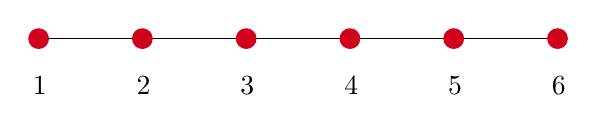
\begin{tikzpicture}[x=0.75pt,y=0.75pt,yscale=-1,xscale=1]
			%uncomment if require: \path (0,300); %set diagram left start at 0, and has height of 300

			%Straight Lines [id:da46250274214576614] 
			\draw    (175,115) -- (425,115) ;
			%Shape: Circle [id:dp08916666481415725] 
			\draw  [draw opacity=0][fill={rgb, 255:red, 208; green, 2; blue, 27 }  ,fill opacity=1 ] (220,115) .. controls (220,112.24) and (222.24,110) .. (225,110) .. controls (227.76,110) and (230,112.24) .. (230,115) .. controls (230,117.76) and (227.76,120) .. (225,120) .. controls (222.24,120) and (220,117.76) .. (220,115) -- cycle ;
			%Shape: Circle [id:dp7997596700799949] 
			\draw  [draw opacity=0][fill={rgb, 255:red, 208; green, 2; blue, 27 }  ,fill opacity=1 ] (270,115) .. controls (270,112.24) and (272.24,110) .. (275,110) .. controls (277.76,110) and (280,112.24) .. (280,115) .. controls (280,117.76) and (277.76,120) .. (275,120) .. controls (272.24,120) and (270,117.76) .. (270,115) -- cycle ;
			%Shape: Circle [id:dp04807433570988917] 
			\draw  [draw opacity=0][fill={rgb, 255:red, 208; green, 2; blue, 27 }  ,fill opacity=1 ] (320,115) .. controls (320,112.24) and (322.24,110) .. (325,110) .. controls (327.76,110) and (330,112.24) .. (330,115) .. controls (330,117.76) and (327.76,120) .. (325,120) .. controls (322.24,120) and (320,117.76) .. (320,115) -- cycle ;
			%Shape: Circle [id:dp6964194673091352] 
			\draw  [draw opacity=0][fill={rgb, 255:red, 208; green, 2; blue, 27 }  ,fill opacity=1 ] (370,115) .. controls (370,112.24) and (372.24,110) .. (375,110) .. controls (377.76,110) and (380,112.24) .. (380,115) .. controls (380,117.76) and (377.76,120) .. (375,120) .. controls (372.24,120) and (370,117.76) .. (370,115) -- cycle ;
			%Shape: Circle [id:dp5929377887646771] 
			\draw  [draw opacity=0][fill={rgb, 255:red, 208; green, 2; blue, 27 }  ,fill opacity=1 ] (420,115) .. controls (420,112.24) and (422.24,110) .. (425,110) .. controls (427.76,110) and (430,112.24) .. (430,115) .. controls (430,117.76) and (427.76,120) .. (425,120) .. controls (422.24,120) and (420,117.76) .. (420,115) -- cycle ;
			%Shape: Circle [id:dp5663003446831361] 
			\draw  [draw opacity=0][fill={rgb, 255:red, 208; green, 2; blue, 27 }  ,fill opacity=1 ] (170,115) .. controls (170,112.24) and (172.24,110) .. (175,110) .. controls (177.76,110) and (180,112.24) .. (180,115) .. controls (180,117.76) and (177.76,120) .. (175,120) .. controls (172.24,120) and (170,117.76) .. (170,115) -- cycle ;

			% Text Node
			\draw (171,132) node [anchor=north west][inner sep=0.75pt]    {$1$};
			% Text Node
			\draw (221,132) node [anchor=north west][inner sep=0.75pt]    {$2$};
			% Text Node
			\draw (271,132) node [anchor=north west][inner sep=0.75pt]    {$3$};
			% Text Node
			\draw (321,132) node [anchor=north west][inner sep=0.75pt]    {$4$};
			% Text Node
			\draw (371,132) node [anchor=north west][inner sep=0.75pt]    {$5$};
			% Text Node
			\draw (421,132) node [anchor=north west][inner sep=0.75pt]    {$6$};


			\end{tikzpicture}

	\end{center}
	This graph is known as $P_6$, a path on 6 vertices.
\end{example}

\subsection{Common Graphs}

There are some graphs that will appear repeatedly throughout the course, and we will define them now.

\begin{definition}[Path]
	We define $P_n$ to be the graph 
	$V = \{1, \dots, n\}$, $E = \{\{1, 2\}, \{2, 3\}, \dots, \{n - 1, n\}\}$ as shown.
	\begin{center}
		

			\tikzset{every picture/.style={line width=0.75pt}} %set default line width to 0.75pt        

			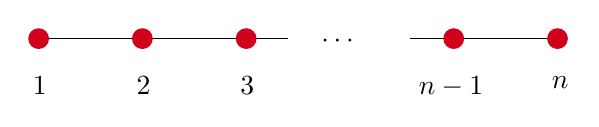
\begin{tikzpicture}[x=0.75pt,y=0.75pt,yscale=-1,xscale=1]
			%uncomment if require: \path (0,93); %set diagram left start at 0, and has height of 93

			%Straight Lines [id:da2966566565444405] 
			\draw    (354,35) -- (425,35) ;
			%Straight Lines [id:da13691249913110026] 
			\draw    (175,35) -- (295,35) ;
			%Shape: Circle [id:dp4038670448284668] 
			\draw  [draw opacity=0][fill={rgb, 255:red, 208; green, 2; blue, 27 }  ,fill opacity=1 ] (220,35) .. controls (220,32.24) and (222.24,30) .. (225,30) .. controls (227.76,30) and (230,32.24) .. (230,35) .. controls (230,37.76) and (227.76,40) .. (225,40) .. controls (222.24,40) and (220,37.76) .. (220,35) -- cycle ;
			%Shape: Circle [id:dp49083678213609794] 
			\draw  [draw opacity=0][fill={rgb, 255:red, 208; green, 2; blue, 27 }  ,fill opacity=1 ] (270,35) .. controls (270,32.24) and (272.24,30) .. (275,30) .. controls (277.76,30) and (280,32.24) .. (280,35) .. controls (280,37.76) and (277.76,40) .. (275,40) .. controls (272.24,40) and (270,37.76) .. (270,35) -- cycle ;
			%Shape: Circle [id:dp06755844317130888] 
			\draw  [draw opacity=0][fill={rgb, 255:red, 208; green, 2; blue, 27 }  ,fill opacity=1 ] (370,35) .. controls (370,32.24) and (372.24,30) .. (375,30) .. controls (377.76,30) and (380,32.24) .. (380,35) .. controls (380,37.76) and (377.76,40) .. (375,40) .. controls (372.24,40) and (370,37.76) .. (370,35) -- cycle ;
			%Shape: Circle [id:dp31955744853716384] 
			\draw  [draw opacity=0][fill={rgb, 255:red, 208; green, 2; blue, 27 }  ,fill opacity=1 ] (420,35) .. controls (420,32.24) and (422.24,30) .. (425,30) .. controls (427.76,30) and (430,32.24) .. (430,35) .. controls (430,37.76) and (427.76,40) .. (425,40) .. controls (422.24,40) and (420,37.76) .. (420,35) -- cycle ;
			%Shape: Circle [id:dp922206172324968] 
			\draw  [draw opacity=0][fill={rgb, 255:red, 208; green, 2; blue, 27 }  ,fill opacity=1 ] (170,35) .. controls (170,32.24) and (172.24,30) .. (175,30) .. controls (177.76,30) and (180,32.24) .. (180,35) .. controls (180,37.76) and (177.76,40) .. (175,40) .. controls (172.24,40) and (170,37.76) .. (170,35) -- cycle ;

			% Text Node
			\draw (171,52) node [anchor=north west][inner sep=0.75pt]    {$1$};
			% Text Node
			\draw (221,52) node [anchor=north west][inner sep=0.75pt]    {$2$};
			% Text Node
			\draw (271,52) node [anchor=north west][inner sep=0.75pt]    {$3$};
			% Text Node
			\draw (357,52) node [anchor=north west][inner sep=0.75pt]    {$n-1$};
			% Text Node
			\draw (421,52) node [anchor=north west][inner sep=0.75pt]    {$n$};
			% Text Node
			\draw (310,32) node [anchor=north west][inner sep=0.75pt]    {$\cdots $};


			\end{tikzpicture}


	\end{center}
	We call this a \vocab{path} on $n$ vertices, and say it has \vocab{length} $n - 1$.
\end{definition}

\begin{definition}[Cycle]
	We define $C_n$ (for $n \geq 3$) to be the graph  $V = \{1, \dots, n\}$, $E = \{ \{1, 2\}, \dots, \{n - 1, n\}, \{n, 1\}\}$ as shown.
	\begin{center}
		
		

\tikzset{every picture/.style={line width=0.75pt}} %set default line width to 0.75pt        

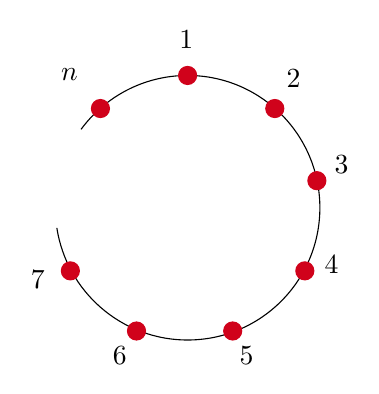
\begin{tikzpicture}[x=0.75pt,y=0.75pt,yscale=-1,xscale=1]
%uncomment if require: \path (0,461); %set diagram left start at 0, and has height of 461

%Shape: Arc [id:dp2939097210495426] 
\draw  [draw opacity=0] (217.92,102.71) .. controls (229.52,86.97) and (248.19,76.75) .. (269.25,76.75) .. controls (304.45,76.75) and (332.98,105.28) .. (332.98,140.48) .. controls (332.98,175.68) and (304.45,204.21) .. (269.25,204.21) .. controls (237.36,204.21) and (210.94,180.77) .. (206.26,150.19) -- (269.25,140.48) -- cycle ; \draw   (217.92,102.71) .. controls (229.52,86.97) and (248.19,76.75) .. (269.25,76.75) .. controls (304.45,76.75) and (332.98,105.28) .. (332.98,140.48) .. controls (332.98,175.68) and (304.45,204.21) .. (269.25,204.21) .. controls (237.36,204.21) and (210.94,180.77) .. (206.26,150.19) ;
%Shape: Ellipse [id:dp08907675877477217] 
\draw  [color={rgb, 255:red, 208; green, 2; blue, 27 }  ,draw opacity=1 ][fill={rgb, 255:red, 208; green, 2; blue, 27 }  ,fill opacity=1 ] (264.91,76.75) .. controls (264.91,74.35) and (266.85,72.41) .. (269.25,72.41) .. controls (271.65,72.41) and (273.6,74.35) .. (273.6,76.75) .. controls (273.6,79.15) and (271.65,81.1) .. (269.25,81.1) .. controls (266.85,81.1) and (264.91,79.15) .. (264.91,76.75) -- cycle ;
%Shape: Ellipse [id:dp6861243810102808] 
\draw  [color={rgb, 255:red, 208; green, 2; blue, 27 }  ,draw opacity=1 ][fill={rgb, 255:red, 208; green, 2; blue, 27 }  ,fill opacity=1 ] (306.91,92.68) .. controls (306.91,90.28) and (308.86,88.34) .. (311.26,88.34) .. controls (313.66,88.34) and (315.6,90.28) .. (315.6,92.68) .. controls (315.6,95.08) and (313.66,97.03) .. (311.26,97.03) .. controls (308.86,97.03) and (306.91,95.08) .. (306.91,92.68) -- cycle ;
%Shape: Circle [id:dp5864785120484053] 
\draw  [color={rgb, 255:red, 208; green, 2; blue, 27 }  ,draw opacity=1 ][fill={rgb, 255:red, 208; green, 2; blue, 27 }  ,fill opacity=1 ] (327.19,127.44) .. controls (327.19,125.04) and (329.13,123.1) .. (331.53,123.1) .. controls (333.93,123.1) and (335.88,125.04) .. (335.88,127.44) .. controls (335.88,129.84) and (333.93,131.79) .. (331.53,131.79) .. controls (329.13,131.79) and (327.19,129.84) .. (327.19,127.44) -- cycle ;
%Shape: Ellipse [id:dp10740847995317393] 
\draw  [color={rgb, 255:red, 208; green, 2; blue, 27 }  ,draw opacity=1 ][fill={rgb, 255:red, 208; green, 2; blue, 27 }  ,fill opacity=1 ] (321.39,170.89) .. controls (321.39,168.5) and (323.34,166.55) .. (325.74,166.55) .. controls (328.14,166.55) and (330.08,168.5) .. (330.08,170.89) .. controls (330.08,173.29) and (328.14,175.24) .. (325.74,175.24) .. controls (323.34,175.24) and (321.39,173.29) .. (321.39,170.89) -- cycle ;
%Shape: Circle [id:dp8188776283145544] 
\draw  [color={rgb, 255:red, 208; green, 2; blue, 27 }  ,draw opacity=1 ][fill={rgb, 255:red, 208; green, 2; blue, 27 }  ,fill opacity=1 ] (286.63,199.86) .. controls (286.63,197.46) and (288.58,195.52) .. (290.98,195.52) .. controls (293.38,195.52) and (295.32,197.46) .. (295.32,199.86) .. controls (295.32,202.26) and (293.38,204.21) .. (290.98,204.21) .. controls (288.58,204.21) and (286.63,202.26) .. (286.63,199.86) -- cycle ;
%Shape: Circle [id:dp20623562846877086] 
\draw  [color={rgb, 255:red, 208; green, 2; blue, 27 }  ,draw opacity=1 ][fill={rgb, 255:red, 208; green, 2; blue, 27 }  ,fill opacity=1 ] (240.29,199.86) .. controls (240.29,197.46) and (242.23,195.52) .. (244.63,195.52) .. controls (247.03,195.52) and (248.98,197.46) .. (248.98,199.86) .. controls (248.98,202.26) and (247.03,204.21) .. (244.63,204.21) .. controls (242.23,204.21) and (240.29,202.26) .. (240.29,199.86) -- cycle ;
%Shape: Ellipse [id:dp8399657424171154] 
\draw  [color={rgb, 255:red, 208; green, 2; blue, 27 }  ,draw opacity=1 ][fill={rgb, 255:red, 208; green, 2; blue, 27 }  ,fill opacity=1 ] (208.42,170.89) .. controls (208.42,168.5) and (210.37,166.55) .. (212.77,166.55) .. controls (215.17,166.55) and (217.11,168.5) .. (217.11,170.89) .. controls (217.11,173.29) and (215.17,175.24) .. (212.77,175.24) .. controls (210.37,175.24) and (208.42,173.29) .. (208.42,170.89) -- cycle ;
%Shape: Rectangle [id:dp758981869824869] 
\draw  [draw opacity=0][fill={rgb, 255:red, 255; green, 255; blue, 255 }  ,fill opacity=0 ] (193.94,99.93) -- (234.49,99.93) -- (234.49,146.27) -- (193.94,146.27) -- cycle ;
%Shape: Ellipse [id:dp07046602779365152] 
\draw  [color={rgb, 255:red, 208; green, 2; blue, 27 }  ,draw opacity=1 ][fill={rgb, 255:red, 208; green, 2; blue, 27 }  ,fill opacity=1 ] (222.91,92.68) .. controls (222.91,90.28) and (224.85,88.34) .. (227.25,88.34) .. controls (229.65,88.34) and (231.6,90.28) .. (231.6,92.68) .. controls (231.6,95.08) and (229.65,97.03) .. (227.25,97.03) .. controls (224.85,97.03) and (222.91,95.08) .. (222.91,92.68) -- cycle ;

% Text Node
\draw (201.99,137.02) node [anchor=north west][inner sep=0.75pt]  [rotate=-289.59]  {$\dotsc $};
% Text Node
\draw (264,54) node [anchor=north west][inner sep=0.75pt]    {$1$};
% Text Node
\draw (315.66,72.55) node [anchor=north west][inner sep=0.75pt]    {$2$};
% Text Node
\draw (338.83,114.1) node [anchor=north west][inner sep=0.75pt]    {$3$};
% Text Node
\draw (334.04,162.45) node [anchor=north west][inner sep=0.75pt]    {$4$};
% Text Node
\draw (293,206) node [anchor=north west][inner sep=0.75pt]    {$5$};
% Text Node
\draw (232.03,206) node [anchor=north west][inner sep=0.75pt]    {$6$};
% Text Node
\draw (192.47,169.45) node [anchor=north west][inner sep=0.75pt]    {$7$};
% Text Node
\draw (207,72) node [anchor=north west][inner sep=0.75pt]    {$n$};


\end{tikzpicture}


	\end{center}
	We call this the \vocab{cycle} on $n$ vertices.
\end{definition}

\begin{definition}[Complete Graph]
	The \vocab{complete graph} on $n$ vertices $K_n$ is the graph $\{1, \dots, n\}$ and $E = \{ \{ i, j \} \mid i \neq j \in V\}$.
	\begin{center}
		

\tikzset{every picture/.style={line width=0.75pt}} %set default line width to 0.75pt        

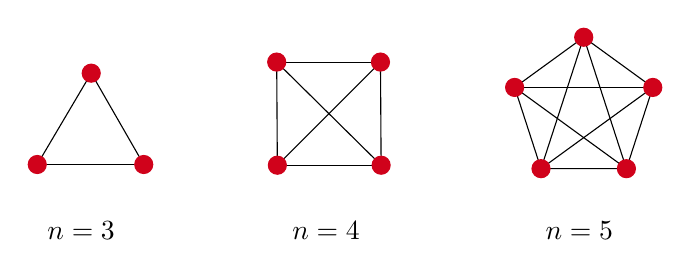
\begin{tikzpicture}[x=0.75pt,y=0.75pt,yscale=-1,xscale=1]
%uncomment if require: \path (0,244); %set diagram left start at 0, and has height of 244

%Straight Lines [id:da9981694225390096] 
\draw    (259.71,56.31) -- (210.02,106) ;
%Straight Lines [id:da26707606947695417] 
\draw    (209.71,56.31) -- (260.02,106) ;
%Straight Lines [id:da6585835091291369] 
\draw    (209.71,56.31) -- (210.02,106) ;
%Straight Lines [id:da7219351678460844] 
\draw    (259.71,56.31) -- (260.02,106) ;
%Straight Lines [id:da0019303873533728089] 
\draw    (209.71,56.31) -- (259.71,56.31) ;
%Straight Lines [id:da7049983363855998] 
\draw    (210.02,106) -- (260.02,106) ;
%Straight Lines [id:da35560926010509697] 
\draw    (120.35,61.65) -- (94.35,105.65) ;
%Straight Lines [id:da7897834071428548] 
\draw    (120.35,61.65) -- (145.65,105.65) ;
%Straight Lines [id:da9938696204324634] 
\draw    (94.35,105.65) -- (145.65,105.65) ;
%Shape: Ellipse [id:dp4113314666492133] 
\draw  [color={rgb, 255:red, 208; green, 2; blue, 27 }  ,draw opacity=1 ][fill={rgb, 255:red, 208; green, 2; blue, 27 }  ,fill opacity=1 ] (90,105.65) .. controls (90,103.26) and (91.95,101.31) .. (94.35,101.31) .. controls (96.74,101.31) and (98.69,103.26) .. (98.69,105.65) .. controls (98.69,108.05) and (96.74,110) .. (94.35,110) .. controls (91.95,110) and (90,108.05) .. (90,105.65) -- cycle ;
%Shape: Ellipse [id:dp834167188739953] 
\draw  [color={rgb, 255:red, 208; green, 2; blue, 27 }  ,draw opacity=1 ][fill={rgb, 255:red, 208; green, 2; blue, 27 }  ,fill opacity=1 ] (141.31,105.65) .. controls (141.31,103.26) and (143.26,101.31) .. (145.65,101.31) .. controls (148.05,101.31) and (150,103.26) .. (150,105.65) .. controls (150,108.05) and (148.05,110) .. (145.65,110) .. controls (143.26,110) and (141.31,108.05) .. (141.31,105.65) -- cycle ;
%Shape: Ellipse [id:dp8095001658436142] 
\draw  [color={rgb, 255:red, 208; green, 2; blue, 27 }  ,draw opacity=1 ][fill={rgb, 255:red, 208; green, 2; blue, 27 }  ,fill opacity=1 ] (116,61.65) .. controls (116,59.26) and (117.95,57.31) .. (120.35,57.31) .. controls (122.74,57.31) and (124.69,59.26) .. (124.69,61.65) .. controls (124.69,64.05) and (122.74,66) .. (120.35,66) .. controls (117.95,66) and (116,64.05) .. (116,61.65) -- cycle ;
%Shape: Ellipse [id:dp10911439146709467] 
\draw  [color={rgb, 255:red, 208; green, 2; blue, 27 }  ,draw opacity=1 ][fill={rgb, 255:red, 208; green, 2; blue, 27 }  ,fill opacity=1 ] (205.37,56.31) .. controls (205.37,53.91) and (207.31,51.96) .. (209.71,51.96) .. controls (212.11,51.96) and (214.06,53.91) .. (214.06,56.31) .. controls (214.06,58.71) and (212.11,60.65) .. (209.71,60.65) .. controls (207.31,60.65) and (205.37,58.71) .. (205.37,56.31) -- cycle ;
%Shape: Ellipse [id:dp8819360357436353] 
\draw  [color={rgb, 255:red, 208; green, 2; blue, 27 }  ,draw opacity=1 ][fill={rgb, 255:red, 208; green, 2; blue, 27 }  ,fill opacity=1 ] (255.37,56.31) .. controls (255.37,53.91) and (257.31,51.96) .. (259.71,51.96) .. controls (262.11,51.96) and (264.06,53.91) .. (264.06,56.31) .. controls (264.06,58.71) and (262.11,60.65) .. (259.71,60.65) .. controls (257.31,60.65) and (255.37,58.71) .. (255.37,56.31) -- cycle ;
%Shape: Ellipse [id:dp05860712986316774] 
\draw  [color={rgb, 255:red, 208; green, 2; blue, 27 }  ,draw opacity=1 ][fill={rgb, 255:red, 208; green, 2; blue, 27 }  ,fill opacity=1 ] (205.68,106) .. controls (205.68,103.6) and (207.62,101.65) .. (210.02,101.65) .. controls (212.42,101.65) and (214.37,103.6) .. (214.37,106) .. controls (214.37,108.4) and (212.42,110.35) .. (210.02,110.35) .. controls (207.62,110.35) and (205.68,108.4) .. (205.68,106) -- cycle ;
%Shape: Ellipse [id:dp5283352169897437] 
\draw  [color={rgb, 255:red, 208; green, 2; blue, 27 }  ,draw opacity=1 ][fill={rgb, 255:red, 208; green, 2; blue, 27 }  ,fill opacity=1 ] (255.68,106) .. controls (255.68,103.6) and (257.62,101.65) .. (260.02,101.65) .. controls (262.42,101.65) and (264.37,103.6) .. (264.37,106) .. controls (264.37,108.4) and (262.42,110.35) .. (260.02,110.35) .. controls (257.62,110.35) and (255.68,108.4) .. (255.68,106) -- cycle ;
%Shape: Regular Polygon [id:dp10308828814670479] 
\draw   (357.63,44.35) -- (390.92,68.53) -- (378.2,107.66) -- (337.06,107.66) -- (324.35,68.53) -- cycle ;
%Straight Lines [id:da43627704398128486] 
\draw    (324.35,68.53) -- (378.2,107.66) ;
%Straight Lines [id:da0011702067257907123] 
\draw    (337.06,107.66) -- (390.92,68.53) ;
%Straight Lines [id:da9427395129530866] 
\draw    (337.06,107.66) -- (357.63,44.35) ;
%Straight Lines [id:da7244564555034867] 
\draw    (324.35,68.53) -- (390.92,68.53) ;
%Straight Lines [id:da6627152022664105] 
\draw    (357.63,44.35) -- (378.2,107.66) ;
%Shape: Ellipse [id:dp7300400411305249] 
\draw  [color={rgb, 255:red, 208; green, 2; blue, 27 }  ,draw opacity=1 ][fill={rgb, 255:red, 208; green, 2; blue, 27 }  ,fill opacity=1 ] (353.29,44.35) .. controls (353.29,41.95) and (355.23,40) .. (357.63,40) .. controls (360.03,40) and (361.98,41.95) .. (361.98,44.35) .. controls (361.98,46.74) and (360.03,48.69) .. (357.63,48.69) .. controls (355.23,48.69) and (353.29,46.74) .. (353.29,44.35) -- cycle ;
%Shape: Ellipse [id:dp8020435268234443] 
\draw  [color={rgb, 255:red, 208; green, 2; blue, 27 }  ,draw opacity=1 ][fill={rgb, 255:red, 208; green, 2; blue, 27 }  ,fill opacity=1 ] (320,68.53) .. controls (320,66.13) and (321.95,64.18) .. (324.35,64.18) .. controls (326.74,64.18) and (328.69,66.13) .. (328.69,68.53) .. controls (328.69,70.93) and (326.74,72.87) .. (324.35,72.87) .. controls (321.95,72.87) and (320,70.93) .. (320,68.53) -- cycle ;
%Shape: Ellipse [id:dp5063058740897554] 
\draw  [color={rgb, 255:red, 208; green, 2; blue, 27 }  ,draw opacity=1 ][fill={rgb, 255:red, 208; green, 2; blue, 27 }  ,fill opacity=1 ] (332.71,107.66) .. controls (332.71,105.26) and (334.66,103.32) .. (337.06,103.32) .. controls (339.46,103.32) and (341.4,105.26) .. (341.4,107.66) .. controls (341.4,110.06) and (339.46,112.01) .. (337.06,112.01) .. controls (334.66,112.01) and (332.71,110.06) .. (332.71,107.66) -- cycle ;
%Shape: Ellipse [id:dp20023345004172588] 
\draw  [color={rgb, 255:red, 208; green, 2; blue, 27 }  ,draw opacity=1 ][fill={rgb, 255:red, 208; green, 2; blue, 27 }  ,fill opacity=1 ] (373.86,107.66) .. controls (373.86,105.26) and (375.8,103.32) .. (378.2,103.32) .. controls (380.6,103.32) and (382.55,105.26) .. (382.55,107.66) .. controls (382.55,110.06) and (380.6,112.01) .. (378.2,112.01) .. controls (375.8,112.01) and (373.86,110.06) .. (373.86,107.66) -- cycle ;
%Shape: Ellipse [id:dp34706748597281534] 
\draw  [color={rgb, 255:red, 208; green, 2; blue, 27 }  ,draw opacity=1 ][fill={rgb, 255:red, 208; green, 2; blue, 27 }  ,fill opacity=1 ] (386.57,68.53) .. controls (386.57,66.13) and (388.52,64.18) .. (390.92,64.18) .. controls (393.32,64.18) and (395.26,66.13) .. (395.26,68.53) .. controls (395.26,70.93) and (393.32,72.87) .. (390.92,72.87) .. controls (388.52,72.87) and (386.57,70.93) .. (386.57,68.53) -- cycle ;

% Text Node
\draw (98,132) node [anchor=north west][inner sep=0.75pt]    {$n=3$};
% Text Node
\draw (216,132) node [anchor=north west][inner sep=0.75pt]    {$n=4$};
% Text Node
\draw (338,132) node [anchor=north west][inner sep=0.75pt]    {$n=5$};


\end{tikzpicture}

	\end{center}
	Note that there is an edge between every pair of vertices.
\end{definition}

\begin{definition}[Empty Graph]
	We define the \vocab{empty graph} on $n$ vertices $\overline{K_n}$ to have $V = \{1, \dots, n\}$ but $E = \emptyset$.
\end{definition}

\begin{remark}
	In our definition of a graph, we {\itshape don't allow} loops, and there {\itshape cannot} be multiple edges between the same set of vertices.
	\begin{center}
		

\tikzset{every picture/.style={line width=0.75pt}} %set default line width to 0.75pt        

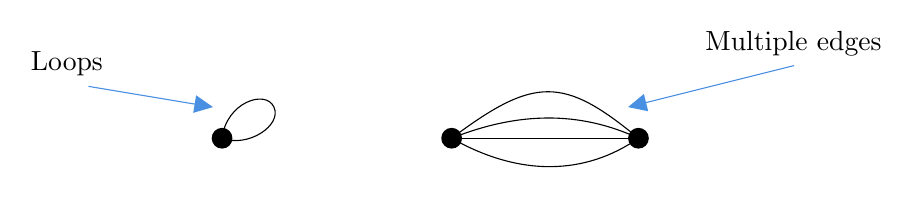
\begin{tikzpicture}[x=0.75pt,y=0.75pt,yscale=-1,xscale=1]
%uncomment if require: \path (0,93); %set diagram left start at 0, and has height of 93

%Curve Lines [id:da2865357772607766] 
\draw    (194.39,55) .. controls (196.39,37.75) and (215.39,31.25) .. (219.39,40) .. controls (223.39,48.75) and (206.89,59.75) .. (194.39,55) -- cycle ;
%Shape: Circle [id:dp0229132580239656] 
\draw  [draw opacity=0][fill={rgb, 255:red, 0; green, 0; blue, 0 }  ,fill opacity=1 ] (189.39,55) .. controls (189.39,52.24) and (191.63,50) .. (194.39,50) .. controls (197.15,50) and (199.39,52.24) .. (199.39,55) .. controls (199.39,57.76) and (197.15,60) .. (194.39,60) .. controls (191.63,60) and (189.39,57.76) .. (189.39,55) -- cycle ;
%Shape: Circle [id:dp1638222573350646] 
\draw  [draw opacity=0][fill={rgb, 255:red, 0; green, 0; blue, 0 }  ,fill opacity=1 ] (300,55) .. controls (300,52.24) and (302.24,50) .. (305,50) .. controls (307.76,50) and (310,52.24) .. (310,55) .. controls (310,57.76) and (307.76,60) .. (305,60) .. controls (302.24,60) and (300,57.76) .. (300,55) -- cycle ;
%Shape: Circle [id:dp537703730076633] 
\draw  [draw opacity=0][fill={rgb, 255:red, 0; green, 0; blue, 0 }  ,fill opacity=1 ] (390,55) .. controls (390,52.24) and (392.24,50) .. (395,50) .. controls (397.76,50) and (400,52.24) .. (400,55) .. controls (400,57.76) and (397.76,60) .. (395,60) .. controls (392.24,60) and (390,57.76) .. (390,55) -- cycle ;
%Straight Lines [id:da6617588206410779] 
\draw    (305,55) -- (395,55) ;
%Curve Lines [id:da23655718519286506] 
\draw    (305,55) .. controls (345,25) and (359,25.25) .. (395,55) ;
%Curve Lines [id:da6706610581979621] 
\draw    (305,55) .. controls (337,42.25) and (366.5,41.75) .. (395,55) ;
%Curve Lines [id:da14619136331292015] 
\draw    (305,55) .. controls (338,73.75) and (369.5,72.75) .. (395,55) ;
%Straight Lines [id:da03138886450780565] 
\draw [color={rgb, 255:red, 74; green, 144; blue, 226 }  ,draw opacity=1 ]   (130,30) -- (187.04,39.51) ;
\draw [shift={(190,40)}, rotate = 189.46] [fill={rgb, 255:red, 74; green, 144; blue, 226 }  ,fill opacity=1 ][line width=0.08]  [draw opacity=0] (8.93,-4.29) -- (0,0) -- (8.93,4.29) -- cycle    ;
%Straight Lines [id:da17643117622964488] 
\draw [color={rgb, 255:red, 74; green, 144; blue, 226 }  ,draw opacity=1 ]   (470,20) -- (392.91,39.27) ;
\draw [shift={(390,40)}, rotate = 345.96000000000004] [fill={rgb, 255:red, 74; green, 144; blue, 226 }  ,fill opacity=1 ][line width=0.08]  [draw opacity=0] (8.93,-4.29) -- (0,0) -- (8.93,4.29) -- cycle    ;

% Text Node
\draw (101,12) node [anchor=north west][inner sep=0.75pt]   [align=left] {Loops};
% Text Node
\draw (426,2) node [anchor=north west][inner sep=0.75pt]   [align=left] {Multiple edges};


\end{tikzpicture}

	\end{center}
	These limitations are inherent in our definition, where we use sets rather than multisets. You can define graphs where such things are allowed, but for now we will outlaw them. We also note that edges are \emph{unordered pairs}, so for now edges have no direction.
\end{remark}

To be slightly more succinct, we will use some shorthand notation. 

\begin{notation}
If $G = (V, E)$ is a graph, and we have some edge $\{x, y\} \in E$, we will denote it by $xy$. We will also define $|G| = |V|$, and $e(G) = |E|$.
\end{notation}
 
\begin{example}[Vertices and Edges of $K_n$]
	Consider the graph $K_n$. We have $|K_n| = n$, and $e(K_n) = \binom{k}{2}$, as there is an edge between any pair of vertices.
\end{example}

\subsection{Subgraphs}

Now we will define the notion of a \emph{subgraph}, in the natural way.

\begin{definition}[Subgraph]
	We say that $H= (V', E')$ is a \vocab{subgraph} of $G = (V, E)$ if $V' \subseteq V$ and $E' \subseteq E$.
\end{definition}

Informally, $H$ is a subgraph of $G$ if we can remove vertices and edges from $G$ to get $H$. Let's look at some examples.

\begin{example}[Example of a Subgraph]
	The graph on the right is a subgraph of the graph on the left.
\begin{center}
	

\tikzset{every picture/.style={line width=0.75pt}} %set default line width to 0.75pt        

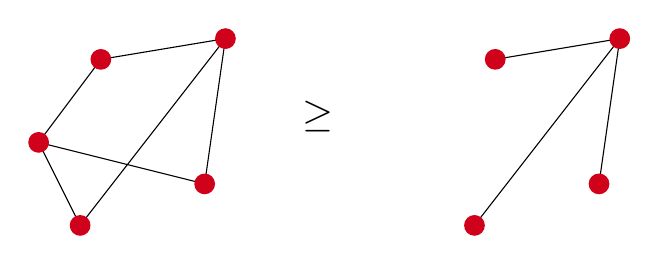
\begin{tikzpicture}[x=0.75pt,y=0.75pt,yscale=-1,xscale=1]
%uncomment if require: \path (0,193); %set diagram left start at 0, and has height of 193

%Straight Lines [id:da5102818539821388] 
\draw    (145,75) -- (175,35) ;
%Straight Lines [id:da11653049971761209] 
\draw    (235,25) -- (175,35) ;
%Straight Lines [id:da5706156443747223] 
\draw    (235,25) -- (225,95) ;
%Straight Lines [id:da9053001100461334] 
\draw    (145,75) -- (165,115) ;
%Straight Lines [id:da5994949539529218] 
\draw    (235,25) -- (165,115) ;
%Straight Lines [id:da2071898142257198] 
\draw    (225,95) -- (145,75) ;
%Shape: Circle [id:dp7335328414030793] 
\draw  [draw opacity=0][fill={rgb, 255:red, 208; green, 2; blue, 27 }  ,fill opacity=1 ] (170,35) .. controls (170,32.24) and (172.24,30) .. (175,30) .. controls (177.76,30) and (180,32.24) .. (180,35) .. controls (180,37.76) and (177.76,40) .. (175,40) .. controls (172.24,40) and (170,37.76) .. (170,35) -- cycle ;
%Shape: Circle [id:dp25158480193801747] 
\draw  [draw opacity=0][fill={rgb, 255:red, 208; green, 2; blue, 27 }  ,fill opacity=1 ] (140,75) .. controls (140,72.24) and (142.24,70) .. (145,70) .. controls (147.76,70) and (150,72.24) .. (150,75) .. controls (150,77.76) and (147.76,80) .. (145,80) .. controls (142.24,80) and (140,77.76) .. (140,75) -- cycle ;
%Shape: Circle [id:dp7366774963822135] 
\draw  [draw opacity=0][fill={rgb, 255:red, 208; green, 2; blue, 27 }  ,fill opacity=1 ] (160,115) .. controls (160,112.24) and (162.24,110) .. (165,110) .. controls (167.76,110) and (170,112.24) .. (170,115) .. controls (170,117.76) and (167.76,120) .. (165,120) .. controls (162.24,120) and (160,117.76) .. (160,115) -- cycle ;
%Shape: Circle [id:dp986170211009179] 
\draw  [draw opacity=0][fill={rgb, 255:red, 208; green, 2; blue, 27 }  ,fill opacity=1 ] (220,95) .. controls (220,92.24) and (222.24,90) .. (225,90) .. controls (227.76,90) and (230,92.24) .. (230,95) .. controls (230,97.76) and (227.76,100) .. (225,100) .. controls (222.24,100) and (220,97.76) .. (220,95) -- cycle ;
%Shape: Circle [id:dp08748002464606974] 
\draw  [draw opacity=0][fill={rgb, 255:red, 208; green, 2; blue, 27 }  ,fill opacity=1 ] (230,25) .. controls (230,22.24) and (232.24,20) .. (235,20) .. controls (237.76,20) and (240,22.24) .. (240,25) .. controls (240,27.76) and (237.76,30) .. (235,30) .. controls (232.24,30) and (230,27.76) .. (230,25) -- cycle ;
%Straight Lines [id:da6558038306138124] 
\draw    (425,25) -- (365,35) ;
%Straight Lines [id:da22960999678468086] 
\draw    (425,25) -- (415,95) ;
%Straight Lines [id:da3699284235556677] 
\draw    (425,25) -- (355,115) ;
%Shape: Circle [id:dp31621516337124767] 
\draw  [draw opacity=0][fill={rgb, 255:red, 208; green, 2; blue, 27 }  ,fill opacity=1 ] (360,35) .. controls (360,32.24) and (362.24,30) .. (365,30) .. controls (367.76,30) and (370,32.24) .. (370,35) .. controls (370,37.76) and (367.76,40) .. (365,40) .. controls (362.24,40) and (360,37.76) .. (360,35) -- cycle ;
%Shape: Circle [id:dp3827184917507753] 
\draw  [draw opacity=0][fill={rgb, 255:red, 208; green, 2; blue, 27 }  ,fill opacity=1 ] (350,115) .. controls (350,112.24) and (352.24,110) .. (355,110) .. controls (357.76,110) and (360,112.24) .. (360,115) .. controls (360,117.76) and (357.76,120) .. (355,120) .. controls (352.24,120) and (350,117.76) .. (350,115) -- cycle ;
%Shape: Circle [id:dp10694204690570841] 
\draw  [draw opacity=0][fill={rgb, 255:red, 208; green, 2; blue, 27 }  ,fill opacity=1 ] (410,95) .. controls (410,92.24) and (412.24,90) .. (415,90) .. controls (417.76,90) and (420,92.24) .. (420,95) .. controls (420,97.76) and (417.76,100) .. (415,100) .. controls (412.24,100) and (410,97.76) .. (410,95) -- cycle ;
%Shape: Circle [id:dp9708117128742255] 
\draw  [draw opacity=0][fill={rgb, 255:red, 208; green, 2; blue, 27 }  ,fill opacity=1 ] (420,25) .. controls (420,22.24) and (422.24,20) .. (425,20) .. controls (427.76,20) and (430,22.24) .. (430,25) .. controls (430,27.76) and (427.76,30) .. (425,30) .. controls (422.24,30) and (420,27.76) .. (420,25) -- cycle ;

% Text Node
\draw (271,54) node [anchor=north west][inner sep=0.75pt]  [font=\Large]  {$\geq $};


\end{tikzpicture}

\end{center}

\end{example}

We are also going to use some notation for removing an edge or a vertex from a graph. Of course, when removing a vertex you also have to remove the edges connecting to it.


\begin{notation}[Adding/Removing Vertices \& Edges]
	For an edge $xy$ or a vertex $x$, we define $G - xy$ to be the graph $G$ with the edge $xy$ removed, and $G - x$ to be $G$ with vertex $x$ removed, along with all edges incident to $x$. We will also define $G + xy$ to be $G$ with the edge $xy$, and $G + x$ to be $G$ with the vertex $x$. 
\end{notation}

\subsection{Graph Isomorphism}

Now that we have defined graphs, it's natural to define some notion of isomorphism.

\begin{definition}[Graph Isomorphism]
	Let $G = (V, E)$ and $H = (V', E')$ be graphs. We say that $f : V \rightarrow V'$ is a \vocab{graph isomorphism} if $f(u)f(v) \in E' \iff uv \in E$. 

	If there is a graph isomorphism between $G$ and $H$ then we say they are \vocab{isomorphic}.
\end{definition}

Now for the following discussion, fix some graph $G = (V, E)$, and let $x \in V$. 

\begin{definition}[Neighbourhood]
	If $xy \in E$, then we say that $x$ and $y$ are \vocab{adjacent}.
	We define the \vocab{neighborhood} of $x$ to be the set $N(x) = \{ y \in V \mid xy \in E\}$ of all vertices adjacent to $x$.
\end{definition}

Note that as in the diagram below, $x$ is not in its own neighborhood.
\begin{center}
	

\tikzset{every picture/.style={line width=0.75pt}} %set default line width to 0.75pt        

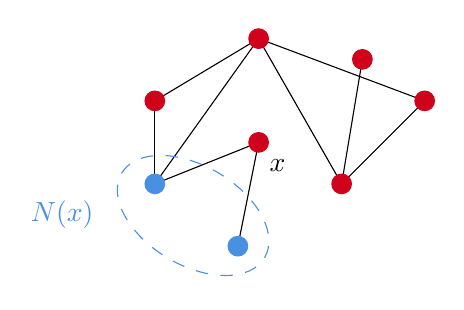
\begin{tikzpicture}[x=0.75pt,y=0.75pt,yscale=-1,xscale=1]
%uncomment if require: \path (0,193); %set diagram left start at 0, and has height of 193

%Straight Lines [id:da9588865668616432] 
\draw    (275,35) -- (225,65) ;
%Straight Lines [id:da6040267926385874] 
\draw    (325,45) -- (315,105) ;
%Straight Lines [id:da2949070003151344] 
\draw    (275,85) -- (265,135) ;
%Straight Lines [id:da20743790772148674] 
\draw    (225,105) -- (275,85) ;
%Straight Lines [id:da4910146433079081] 
\draw    (225,105) -- (225,65) ;
%Straight Lines [id:da5820247237359314] 
\draw    (225,105) -- (275,35) ;
%Straight Lines [id:da5614914262150004] 
\draw    (275,35) -- (315,105) ;
%Straight Lines [id:da23660182919629502] 
\draw    (355,65) -- (275,35) ;
%Straight Lines [id:da18662720934380073] 
\draw    (355,65) -- (315,105) ;
%Shape: Circle [id:dp7796053805504014] 
\draw  [draw opacity=0][fill={rgb, 255:red, 208; green, 2; blue, 27 }  ,fill opacity=1 ] (220,65) .. controls (220,62.24) and (222.24,60) .. (225,60) .. controls (227.76,60) and (230,62.24) .. (230,65) .. controls (230,67.76) and (227.76,70) .. (225,70) .. controls (222.24,70) and (220,67.76) .. (220,65) -- cycle ;
%Shape: Circle [id:dp5410193836574619] 
\draw  [draw opacity=0][fill={rgb, 255:red, 208; green, 2; blue, 27 }  ,fill opacity=1 ] (270,35) .. controls (270,32.24) and (272.24,30) .. (275,30) .. controls (277.76,30) and (280,32.24) .. (280,35) .. controls (280,37.76) and (277.76,40) .. (275,40) .. controls (272.24,40) and (270,37.76) .. (270,35) -- cycle ;
%Shape: Circle [id:dp7645390851559083] 
\draw  [draw opacity=0][fill={rgb, 255:red, 208; green, 2; blue, 27 }  ,fill opacity=1 ] (320,45) .. controls (320,42.24) and (322.24,40) .. (325,40) .. controls (327.76,40) and (330,42.24) .. (330,45) .. controls (330,47.76) and (327.76,50) .. (325,50) .. controls (322.24,50) and (320,47.76) .. (320,45) -- cycle ;
%Shape: Circle [id:dp2737498580146679] 
\draw  [draw opacity=0][fill={rgb, 255:red, 74; green, 144; blue, 226 }  ,fill opacity=1 ] (220,105) .. controls (220,102.24) and (222.24,100) .. (225,100) .. controls (227.76,100) and (230,102.24) .. (230,105) .. controls (230,107.76) and (227.76,110) .. (225,110) .. controls (222.24,110) and (220,107.76) .. (220,105) -- cycle ;
%Shape: Circle [id:dp8649705530172823] 
\draw  [draw opacity=0][fill={rgb, 255:red, 208; green, 2; blue, 27 }  ,fill opacity=1 ] (270,85) .. controls (270,82.24) and (272.24,80) .. (275,80) .. controls (277.76,80) and (280,82.24) .. (280,85) .. controls (280,87.76) and (277.76,90) .. (275,90) .. controls (272.24,90) and (270,87.76) .. (270,85) -- cycle ;
%Shape: Circle [id:dp37860744340197594] 
\draw  [draw opacity=0][fill={rgb, 255:red, 208; green, 2; blue, 27 }  ,fill opacity=1 ] (310,105) .. controls (310,102.24) and (312.24,100) .. (315,100) .. controls (317.76,100) and (320,102.24) .. (320,105) .. controls (320,107.76) and (317.76,110) .. (315,110) .. controls (312.24,110) and (310,107.76) .. (310,105) -- cycle ;
%Shape: Circle [id:dp16994333406917272] 
\draw  [draw opacity=0][fill={rgb, 255:red, 74; green, 144; blue, 226 }  ,fill opacity=1 ] (260,135) .. controls (260,132.24) and (262.24,130) .. (265,130) .. controls (267.76,130) and (270,132.24) .. (270,135) .. controls (270,137.76) and (267.76,140) .. (265,140) .. controls (262.24,140) and (260,137.76) .. (260,135) -- cycle ;
%Shape: Circle [id:dp7574466548746062] 
\draw  [draw opacity=0][fill={rgb, 255:red, 208; green, 2; blue, 27 }  ,fill opacity=1 ] (350,65) .. controls (350,62.24) and (352.24,60) .. (355,60) .. controls (357.76,60) and (360,62.24) .. (360,65) .. controls (360,67.76) and (357.76,70) .. (355,70) .. controls (352.24,70) and (350,67.76) .. (350,65) -- cycle ;
%Shape: Ellipse [id:dp42082831262373377] 
\draw  [color={rgb, 255:red, 74; green, 144; blue, 226 }  ,draw opacity=1 ][dash pattern={on 4.5pt off 4.5pt}] (208.98,99.87) .. controls (215.68,88.53) and (236.53,88.43) .. (255.56,99.66) .. controls (274.58,110.89) and (284.57,129.2) .. (277.87,140.55) .. controls (271.17,151.9) and (250.31,151.99) .. (231.29,140.76) .. controls (212.27,129.53) and (202.28,111.22) .. (208.98,99.87) -- cycle ;

% Text Node
\draw (279,92) node [anchor=north west][inner sep=0.75pt]    {$x$};
% Text Node
\draw (164,112) node [anchor=north west][inner sep=0.75pt]  [color={rgb, 255:red, 74; green, 144; blue, 226 }  ,opacity=1 ]  {$N( x)$};


\end{tikzpicture}

\end{center}

\begin{definition}[Degree]
	We define the \vocab{degree} of a vertex $x$ to be $d(x) = |N(x)|$. This is equal to the number of edges that are incident to $x$.
\end{definition}

% Now for some graph $G$ with vertices $V = \{x_1, \dots, x_n\}$, we say the \vocab{degree sequence} of $G$ is $d(x_1), d(x_2), \dots, d(x_n)$.

\begin{definition}[Regularity]
	A graph $G$ is said to be \vocab{regular} if all of the degrees are the same. We say $G$ is $k$-regular if $d(x) = k$ for all $x \in V$.
\end{definition}

\begin{example}[Regular and Non-Regular Graphs]
	The graphs $K_n$ is $n - 1$ regular, and $C_n$ is $2$-regular.
	The graph $P_n$ is not regular.
\end{example}

\subsection{Connectivity}

We now want to define some notion of \emph{connectivity}, where a vertex $u$ is connected to vertex $v$ if you can follow some path in the graph to get from $u$ to $v$.

\begin{center}

	

\tikzset{every picture/.style={line width=0.75pt}} %set default line width to 0.75pt        

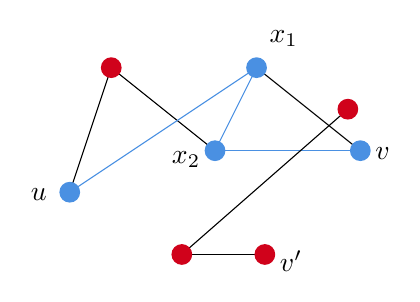
\begin{tikzpicture}[x=0.75pt,y=0.75pt,yscale=-1,xscale=1]
%uncomment if require: \path (0,193); %set diagram left start at 0, and has height of 193

%Straight Lines [id:da622057432821673] 
\draw    (211,75) -- (231,15) ;
%Straight Lines [id:da45132208780914207] 
\draw    (231,15) -- (281,55) ;
%Straight Lines [id:da30820364060918315] 
\draw [color={rgb, 255:red, 74; green, 144; blue, 226 }  ,draw opacity=1 ]   (301,15) -- (281,55) ;
%Straight Lines [id:da8027434077669512] 
\draw [color={rgb, 255:red, 74; green, 144; blue, 226 }  ,draw opacity=1 ]   (351,55) -- (281,55) ;
%Straight Lines [id:da16630547460303047] 
\draw [color={rgb, 255:red, 74; green, 144; blue, 226 }  ,draw opacity=1 ]   (301,15) -- (211,75) ;
%Straight Lines [id:da9414715970752923] 
\draw    (351,55) -- (301,15) ;
%Straight Lines [id:da009376398482458415] 
\draw    (345,35) -- (265,105) ;
%Straight Lines [id:da8452379949704987] 
\draw    (305,105) -- (265,105) ;
%Shape: Circle [id:dp8926415649677933] 
\draw  [draw opacity=0][fill={rgb, 255:red, 208; green, 2; blue, 27 }  ,fill opacity=1 ] (226,15) .. controls (226,12.24) and (228.24,10) .. (231,10) .. controls (233.76,10) and (236,12.24) .. (236,15) .. controls (236,17.76) and (233.76,20) .. (231,20) .. controls (228.24,20) and (226,17.76) .. (226,15) -- cycle ;
%Shape: Circle [id:dp06866505571224346] 
\draw  [draw opacity=0][fill={rgb, 255:red, 74; green, 144; blue, 226 }  ,fill opacity=1 ] (296,15) .. controls (296,12.24) and (298.24,10) .. (301,10) .. controls (303.76,10) and (306,12.24) .. (306,15) .. controls (306,17.76) and (303.76,20) .. (301,20) .. controls (298.24,20) and (296,17.76) .. (296,15) -- cycle ;
%Shape: Circle [id:dp3115374601380443] 
\draw  [draw opacity=0][fill={rgb, 255:red, 74; green, 144; blue, 226 }  ,fill opacity=1 ] (206,75) .. controls (206,72.24) and (208.24,70) .. (211,70) .. controls (213.76,70) and (216,72.24) .. (216,75) .. controls (216,77.76) and (213.76,80) .. (211,80) .. controls (208.24,80) and (206,77.76) .. (206,75) -- cycle ;
%Shape: Circle [id:dp14211747814115727] 
\draw  [draw opacity=0][fill={rgb, 255:red, 74; green, 144; blue, 226 }  ,fill opacity=1 ] (346,55) .. controls (346,52.24) and (348.24,50) .. (351,50) .. controls (353.76,50) and (356,52.24) .. (356,55) .. controls (356,57.76) and (353.76,60) .. (351,60) .. controls (348.24,60) and (346,57.76) .. (346,55) -- cycle ;
%Shape: Circle [id:dp9991626952144155] 
\draw  [draw opacity=0][fill={rgb, 255:red, 74; green, 144; blue, 226 }  ,fill opacity=1 ] (276,55) .. controls (276,52.24) and (278.24,50) .. (281,50) .. controls (283.76,50) and (286,52.24) .. (286,55) .. controls (286,57.76) and (283.76,60) .. (281,60) .. controls (278.24,60) and (276,57.76) .. (276,55) -- cycle ;
%Shape: Circle [id:dp5747900065455143] 
\draw  [draw opacity=0][fill={rgb, 255:red, 208; green, 2; blue, 27 }  ,fill opacity=1 ] (300,105) .. controls (300,102.24) and (302.24,100) .. (305,100) .. controls (307.76,100) and (310,102.24) .. (310,105) .. controls (310,107.76) and (307.76,110) .. (305,110) .. controls (302.24,110) and (300,107.76) .. (300,105) -- cycle ;
%Shape: Circle [id:dp13737323142390678] 
\draw  [draw opacity=0][fill={rgb, 255:red, 208; green, 2; blue, 27 }  ,fill opacity=1 ] (260,105) .. controls (260,102.24) and (262.24,100) .. (265,100) .. controls (267.76,100) and (270,102.24) .. (270,105) .. controls (270,107.76) and (267.76,110) .. (265,110) .. controls (262.24,110) and (260,107.76) .. (260,105) -- cycle ;
%Shape: Circle [id:dp04201057706920763] 
\draw  [draw opacity=0][fill={rgb, 255:red, 208; green, 2; blue, 27 }  ,fill opacity=1 ] (340,35) .. controls (340,32.24) and (342.24,30) .. (345,30) .. controls (347.76,30) and (350,32.24) .. (350,35) .. controls (350,37.76) and (347.76,40) .. (345,40) .. controls (342.24,40) and (340,37.76) .. (340,35) -- cycle ;

% Text Node
\draw (191,72) node [anchor=north west][inner sep=0.75pt]    {$u$};
% Text Node
\draw (357,52) node [anchor=north west][inner sep=0.75pt]    {$v$};
% Text Node
\draw (311,102) node [anchor=north west][inner sep=0.75pt]    {$v'$};
% Text Node
\draw (259,54) node [anchor=north west][inner sep=0.75pt]    {$x_{2}$};
% Text Node
\draw (306,-4) node [anchor=north west][inner sep=0.75pt]    {$x_{1}$};


\end{tikzpicture}


\end{center}

For example, in the graph above we want to say somehow that $u$ and $v$ are connected, but $u$ and $v'$ are not. To do this, we will introduce some more definitions.

\begin{definition}[$uv$ Path]
	A \vocab{$uv$ path} is a sequence $x_1, x_2, \dots, x_l$ where $x_1, \dots, x_l$ are distinct, $x_1 = u$, $x_l = v$ and $x_i x_{i + 1} \in E$.
\end{definition}

In the example above, $u x_1 x_2 v$ is a $uv$ path. 

The slight subtlety in this condition is the \emph{distinctness} condition. For example, if $x_1 \dots x_l$ is a $uv$ path and $y_1 \dots y_{l'}$ is a $vw$ path, then $x_1 \dots x_l y_1 \dots y_{l'}$ may \emph{not} be a $uw$ path since we may have reused an edge. Of course, we can just not reuse edges by avoiding cycles.

\begin{proposition}[Joining Paths]
	If $x_1 \dots x_l$ is a $uv$ path and $y_1 \dots y_{l'}$ is a $vw$ path, then $x_1 \dots x_l y_1 \dots y_{l'}$ contains a $uw$ path.
\end{proposition}
\begin{proof}
	Choose a minimal subsequence $w_1 \dots w_r$ of $x_1 \dots x_l y_1 \dots y_{l'}$ such that
	\begin{enumerate}
		\item $w_i w_{i + 1} \in E$.
		\item $w_1 = u$, $w_r = w$.
	\end{enumerate}
	We now claim that $w_1 \dots w_r$ is a $uw$ path. If this was not the case, then it must fail on distinctness, so there would exist some $z$ such that the sequence is
	$$
	w_1 \dots w_{a} z w_{a + 2} \dots w_b z w_{b + 2} w_r,
	$$
	but now note that
	$$
	w_1 \dots w_{a}zw_{b+2} \dots w_r
	$$
	also satisfies the conditions for the subsequence, but is strictly shorter length. This contradicts the minimality condition.
\end{proof}

Now given $G = (V, E)$, let's define an equivalence relation $\sim$ on $V$, where
$$
x \sim y \iff \text{there exists an $xy$ path in $G$}.
$$

\begin{proposition}
	$\sim$ is an equivalence relation.
\end{proposition}
\begin{proof}
	Note that $\sim$ is reflexive and symmetric, and we get transitivity from our previous proposition.
\end{proof}


\begin{example}
	In the graph below, the vertices that are the same colour are in the same equivalence class under $\sim$.
	\begin{center}
		

\tikzset{every picture/.style={line width=0.75pt}} %set default line width to 0.75pt        

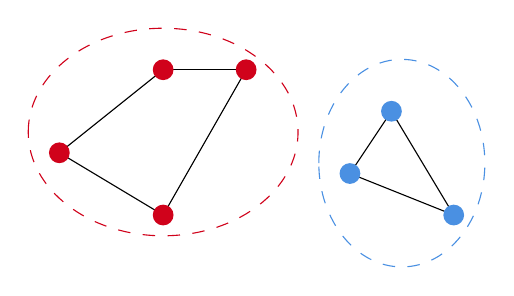
\begin{tikzpicture}[x=0.75pt,y=0.75pt,yscale=-1,xscale=1]
%uncomment if require: \path (0,193); %set diagram left start at 0, and has height of 193

%Straight Lines [id:da026420751885910643] 
\draw    (235,55) -- (185,95) ;
%Straight Lines [id:da9722690765704908] 
\draw    (275,55) -- (235,55) ;
%Straight Lines [id:da06843618607928192] 
\draw    (235,125) -- (275,55) ;
%Straight Lines [id:da5625605688196442] 
\draw    (185,95) -- (235,125) ;
%Straight Lines [id:da988200478921885] 
\draw    (325,105) -- (345,75) ;
%Straight Lines [id:da911347603435119] 
\draw    (375,125) -- (345,75) ;
%Straight Lines [id:da8522085082708648] 
\draw    (375,125) -- (325,105) ;
%Shape: Circle [id:dp6731202040761254] 
\draw  [draw opacity=0][fill={rgb, 255:red, 74; green, 144; blue, 226 }  ,fill opacity=1 ] (320,105) .. controls (320,102.24) and (322.24,100) .. (325,100) .. controls (327.76,100) and (330,102.24) .. (330,105) .. controls (330,107.76) and (327.76,110) .. (325,110) .. controls (322.24,110) and (320,107.76) .. (320,105) -- cycle ;
%Shape: Circle [id:dp6918700817283945] 
\draw  [draw opacity=0][fill={rgb, 255:red, 74; green, 144; blue, 226 }  ,fill opacity=1 ] (340,75) .. controls (340,72.24) and (342.24,70) .. (345,70) .. controls (347.76,70) and (350,72.24) .. (350,75) .. controls (350,77.76) and (347.76,80) .. (345,80) .. controls (342.24,80) and (340,77.76) .. (340,75) -- cycle ;
%Shape: Circle [id:dp8990189535612337] 
\draw  [draw opacity=0][fill={rgb, 255:red, 74; green, 144; blue, 226 }  ,fill opacity=1 ] (370,125) .. controls (370,122.24) and (372.24,120) .. (375,120) .. controls (377.76,120) and (380,122.24) .. (380,125) .. controls (380,127.76) and (377.76,130) .. (375,130) .. controls (372.24,130) and (370,127.76) .. (370,125) -- cycle ;
%Shape: Circle [id:dp5598547497180938] 
\draw  [draw opacity=0][fill={rgb, 255:red, 208; green, 2; blue, 27 }  ,fill opacity=1 ] (230,55) .. controls (230,52.24) and (232.24,50) .. (235,50) .. controls (237.76,50) and (240,52.24) .. (240,55) .. controls (240,57.76) and (237.76,60) .. (235,60) .. controls (232.24,60) and (230,57.76) .. (230,55) -- cycle ;
%Shape: Circle [id:dp38539457383955944] 
\draw  [draw opacity=0][fill={rgb, 255:red, 208; green, 2; blue, 27 }  ,fill opacity=1 ] (180,95) .. controls (180,92.24) and (182.24,90) .. (185,90) .. controls (187.76,90) and (190,92.24) .. (190,95) .. controls (190,97.76) and (187.76,100) .. (185,100) .. controls (182.24,100) and (180,97.76) .. (180,95) -- cycle ;
%Shape: Circle [id:dp7818087689592826] 
\draw  [draw opacity=0][fill={rgb, 255:red, 208; green, 2; blue, 27 }  ,fill opacity=1 ] (230,125) .. controls (230,122.24) and (232.24,120) .. (235,120) .. controls (237.76,120) and (240,122.24) .. (240,125) .. controls (240,127.76) and (237.76,130) .. (235,130) .. controls (232.24,130) and (230,127.76) .. (230,125) -- cycle ;
%Shape: Circle [id:dp7622426997206498] 
\draw  [draw opacity=0][fill={rgb, 255:red, 208; green, 2; blue, 27 }  ,fill opacity=1 ] (270,55) .. controls (270,52.24) and (272.24,50) .. (275,50) .. controls (277.76,50) and (280,52.24) .. (280,55) .. controls (280,57.76) and (277.76,60) .. (275,60) .. controls (272.24,60) and (270,57.76) .. (270,55) -- cycle ;
%Shape: Ellipse [id:dp39967148726972657] 
\draw  [color={rgb, 255:red, 208; green, 2; blue, 27 }  ,draw opacity=1 ][dash pattern={on 4.5pt off 4.5pt}] (170,85) .. controls (170,57.39) and (199.1,35) .. (235,35) .. controls (270.9,35) and (300,57.39) .. (300,85) .. controls (300,112.61) and (270.9,135) .. (235,135) .. controls (199.1,135) and (170,112.61) .. (170,85) -- cycle ;
%Shape: Ellipse [id:dp994417464374959] 
\draw  [color={rgb, 255:red, 74; green, 144; blue, 226 }  ,draw opacity=1 ][dash pattern={on 4.5pt off 4.5pt}] (310,100) .. controls (310,72.39) and (327.91,50) .. (350,50) .. controls (372.09,50) and (390,72.39) .. (390,100) .. controls (390,127.61) and (372.09,150) .. (350,150) .. controls (327.91,150) and (310,127.61) .. (310,100) -- cycle ;




\end{tikzpicture}

	\end{center}
\end{example}

\begin{definition}[Connected Graph]
If there is a path between any two vertices in $G$ then we say that $G$ is \vocab{connected}.	
\end{definition}

\begin{definition}[Connected Components]
We call the equivalence classes of $\sim$ on $G$ the \vocab{components} or \vocab{connected components} of $G$.
\end{definition}

\subsection{Edges and Distance}

We can also introduce some useful definitions relating to the edges of a graph.

\begin{definition}[Minimum/Maximum Degree]
	Let $G$ be a graph. The \vocab{maximum degree} of $G$, $\triangle(G)$ is defined to be $\triangle(G) = \max_{x \in V} d(x)$. Similarly, we define the \vocab{minimum degree} of $G$, $\delta(G)$ to be $\delta(G) = \min_{x \in V} d(x)$.
\end{definition}

In a $k$-regular graph as mentioned above, we have $\triangle(G) = \delta(G) = k$.

\begin{definition}[Graph Distance]
Let $G = (V, E)$ be a graph. The associated \vocab{graph distance} $d: V \times V \rightarrow \R^{\geq 0} \cup \{ \infty \}$ is defined so that $d(x, y)$ is the minimum path length from $x$ to $y$ if it exists, and $\infty$ otherwise.
\end{definition}

\begin{proposition}[Graph Distance is a Metric]
	Let $G = (V, E)$ be a connected graph and let $d$ be the associated graph distance. Then $(V, d)$ defines a metric space.
\end{proposition}
\begin{proof}[Proof Sketch]
	We have $d(x, y) = 0$, and $d(x, y) = d(y, x)$ (taking the shortest path in the opposite direction), and $d(x, z) \leq d(x, y) + d(y, z)$ as we can find path from $x$ to $z$ by taking paths from $x$ to $y$ and $y$ to $z$ and adjoining them, and this puts an upper bound on $d(x, z)$.
\end{proof}

\section{Trees}

We will now discuss a special class of graph called \emph{trees}.
This class is quite restrictive (yet is quite useful), and they have some nice properties.

To define what a tree is, we first need a notion of when a graph is acyclic.

\begin{definition}[Acyclic]
	A graph $G$ is said to be \vocab{acyclic} if it does not contain any subgraph isomorphic to a cycle, $C_n$.
\end{definition}

\begin{example}[Example of Acyclic/Non-Acyclic Graphs]
	In the example below, the two graphs are both \emph{acyclic}.
	\begin{center}


		\tikzset{every picture/.style={line width=0.75pt}} %set default line width to 0.75pt        

		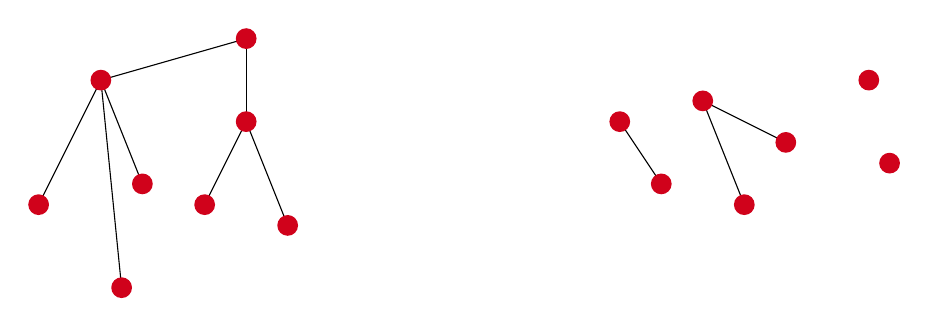
\begin{tikzpicture}[x=0.75pt,y=0.75pt,yscale=-1,xscale=1]
		%uncomment if require: \path (0,193); %set diagram left start at 0, and has height of 193
		
		%Straight Lines [id:da4975879578224476] 
		\draw    (195,25) -- (125,45) ;
		%Straight Lines [id:da9875182002621871] 
		\draw    (195,25) -- (195,65) ;
		%Straight Lines [id:da14692421279536638] 
		\draw    (125,45) -- (145,95) ;
		%Straight Lines [id:da5597906353336949] 
		\draw    (125,45) -- (135,145) ;
		%Straight Lines [id:da827590697469549] 
		\draw    (125,45) -- (95,105) ;
		%Straight Lines [id:da24566898686094285] 
		\draw    (195,65) -- (175,105) ;
		%Straight Lines [id:da013473140578307952] 
		\draw    (195,65) -- (215,115) ;
		%Shape: Circle [id:dp017139343550431563] 
		\draw  [draw opacity=0][fill={rgb, 255:red, 208; green, 2; blue, 27 }  ,fill opacity=1 ] (120,45) .. controls (120,42.24) and (122.24,40) .. (125,40) .. controls (127.76,40) and (130,42.24) .. (130,45) .. controls (130,47.76) and (127.76,50) .. (125,50) .. controls (122.24,50) and (120,47.76) .. (120,45) -- cycle ;
		%Shape: Circle [id:dp9218534791001208] 
		\draw  [draw opacity=0][fill={rgb, 255:red, 208; green, 2; blue, 27 }  ,fill opacity=1 ] (190,25) .. controls (190,22.24) and (192.24,20) .. (195,20) .. controls (197.76,20) and (200,22.24) .. (200,25) .. controls (200,27.76) and (197.76,30) .. (195,30) .. controls (192.24,30) and (190,27.76) .. (190,25) -- cycle ;
		%Shape: Circle [id:dp2781242473026011] 
		\draw  [draw opacity=0][fill={rgb, 255:red, 208; green, 2; blue, 27 }  ,fill opacity=1 ] (190,65) .. controls (190,62.24) and (192.24,60) .. (195,60) .. controls (197.76,60) and (200,62.24) .. (200,65) .. controls (200,67.76) and (197.76,70) .. (195,70) .. controls (192.24,70) and (190,67.76) .. (190,65) -- cycle ;
		%Shape: Circle [id:dp030803892200315652] 
		\draw  [draw opacity=0][fill={rgb, 255:red, 208; green, 2; blue, 27 }  ,fill opacity=1 ] (90,105) .. controls (90,102.24) and (92.24,100) .. (95,100) .. controls (97.76,100) and (100,102.24) .. (100,105) .. controls (100,107.76) and (97.76,110) .. (95,110) .. controls (92.24,110) and (90,107.76) .. (90,105) -- cycle ;
		%Shape: Circle [id:dp05177451328998328] 
		\draw  [draw opacity=0][fill={rgb, 255:red, 208; green, 2; blue, 27 }  ,fill opacity=1 ] (130,145) .. controls (130,142.24) and (132.24,140) .. (135,140) .. controls (137.76,140) and (140,142.24) .. (140,145) .. controls (140,147.76) and (137.76,150) .. (135,150) .. controls (132.24,150) and (130,147.76) .. (130,145) -- cycle ;
		%Shape: Circle [id:dp9829721568494545] 
		\draw  [draw opacity=0][fill={rgb, 255:red, 208; green, 2; blue, 27 }  ,fill opacity=1 ] (140,95) .. controls (140,92.24) and (142.24,90) .. (145,90) .. controls (147.76,90) and (150,92.24) .. (150,95) .. controls (150,97.76) and (147.76,100) .. (145,100) .. controls (142.24,100) and (140,97.76) .. (140,95) -- cycle ;
		%Shape: Circle [id:dp41010913556293216] 
		\draw  [draw opacity=0][fill={rgb, 255:red, 208; green, 2; blue, 27 }  ,fill opacity=1 ] (210,115) .. controls (210,112.24) and (212.24,110) .. (215,110) .. controls (217.76,110) and (220,112.24) .. (220,115) .. controls (220,117.76) and (217.76,120) .. (215,120) .. controls (212.24,120) and (210,117.76) .. (210,115) -- cycle ;
		%Shape: Circle [id:dp2845228574030323] 
		\draw  [draw opacity=0][fill={rgb, 255:red, 208; green, 2; blue, 27 }  ,fill opacity=1 ] (170,105) .. controls (170,102.24) and (172.24,100) .. (175,100) .. controls (177.76,100) and (180,102.24) .. (180,105) .. controls (180,107.76) and (177.76,110) .. (175,110) .. controls (172.24,110) and (170,107.76) .. (170,105) -- cycle ;
		%Straight Lines [id:da3465675313818486] 
		\draw    (415,55) -- (435,105) ;
		%Shape: Circle [id:dp4803286610625792] 
		\draw  [draw opacity=0][fill={rgb, 255:red, 208; green, 2; blue, 27 }  ,fill opacity=1 ] (430,105) .. controls (430,102.24) and (432.24,100) .. (435,100) .. controls (437.76,100) and (440,102.24) .. (440,105) .. controls (440,107.76) and (437.76,110) .. (435,110) .. controls (432.24,110) and (430,107.76) .. (430,105) -- cycle ;
		%Straight Lines [id:da21407762828429155] 
		\draw    (415,55) -- (455,75) ;
		%Shape: Circle [id:dp6332637183866524] 
		\draw  [draw opacity=0][fill={rgb, 255:red, 208; green, 2; blue, 27 }  ,fill opacity=1 ] (450,75) .. controls (450,72.24) and (452.24,70) .. (455,70) .. controls (457.76,70) and (460,72.24) .. (460,75) .. controls (460,77.76) and (457.76,80) .. (455,80) .. controls (452.24,80) and (450,77.76) .. (450,75) -- cycle ;
		%Shape: Circle [id:dp7070779056968607] 
		\draw  [draw opacity=0][fill={rgb, 255:red, 208; green, 2; blue, 27 }  ,fill opacity=1 ] (410,55) .. controls (410,52.24) and (412.24,50) .. (415,50) .. controls (417.76,50) and (420,52.24) .. (420,55) .. controls (420,57.76) and (417.76,60) .. (415,60) .. controls (412.24,60) and (410,57.76) .. (410,55) -- cycle ;
		%Shape: Circle [id:dp5461528770985675] 
		\draw  [draw opacity=0][fill={rgb, 255:red, 208; green, 2; blue, 27 }  ,fill opacity=1 ] (500,85) .. controls (500,82.24) and (502.24,80) .. (505,80) .. controls (507.76,80) and (510,82.24) .. (510,85) .. controls (510,87.76) and (507.76,90) .. (505,90) .. controls (502.24,90) and (500,87.76) .. (500,85) -- cycle ;
		%Shape: Circle [id:dp2134597956334484] 
		\draw  [draw opacity=0][fill={rgb, 255:red, 208; green, 2; blue, 27 }  ,fill opacity=1 ] (490,45) .. controls (490,42.24) and (492.24,40) .. (495,40) .. controls (497.76,40) and (500,42.24) .. (500,45) .. controls (500,47.76) and (497.76,50) .. (495,50) .. controls (492.24,50) and (490,47.76) .. (490,45) -- cycle ;
		%Straight Lines [id:da9266795704990405] 
		\draw    (375,65) -- (395,95) ;
		%Shape: Circle [id:dp5484535938793745] 
		\draw  [draw opacity=0][fill={rgb, 255:red, 208; green, 2; blue, 27 }  ,fill opacity=1 ] (390,95) .. controls (390,92.24) and (392.24,90) .. (395,90) .. controls (397.76,90) and (400,92.24) .. (400,95) .. controls (400,97.76) and (397.76,100) .. (395,100) .. controls (392.24,100) and (390,97.76) .. (390,95) -- cycle ;
		%Shape: Circle [id:dp9664538152744377] 
		\draw  [draw opacity=0][fill={rgb, 255:red, 208; green, 2; blue, 27 }  ,fill opacity=1 ] (370,65) .. controls (370,62.24) and (372.24,60) .. (375,60) .. controls (377.76,60) and (380,62.24) .. (380,65) .. controls (380,67.76) and (377.76,70) .. (375,70) .. controls (372.24,70) and (370,67.76) .. (370,65) -- cycle ;
		
		
		
		
		\end{tikzpicture}
		
	\end{center}
Two \emph{non-acyclic} graphs are shown below. The subgraphs isomorphic to $C_4$ and $C_3$ are highlighted.
\begin{center}
	\tikzset{every picture/.style={line width=0.75pt}} %set default line width to 0.75pt        

	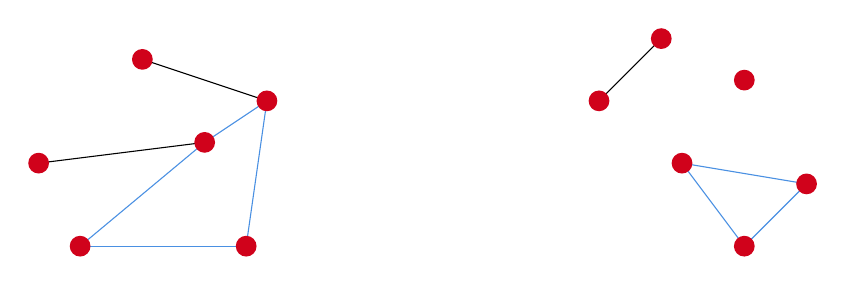
\begin{tikzpicture}[x=0.75pt,y=0.75pt,yscale=-1,xscale=1]
	%uncomment if require: \path (0,193); %set diagram left start at 0, and has height of 193
	
	%Shape: Circle [id:dp866182978887481] 
	\draw  [draw opacity=0][fill={rgb, 255:red, 208; green, 2; blue, 27 }  ,fill opacity=1 ] (490,45) .. controls (490,42.24) and (492.24,40) .. (495,40) .. controls (497.76,40) and (500,42.24) .. (500,45) .. controls (500,47.76) and (497.76,50) .. (495,50) .. controls (492.24,50) and (490,47.76) .. (490,45) -- cycle ;
	%Straight Lines [id:da3990958073757699] 
	\draw    (205,35) -- (265,55) ;
	%Straight Lines [id:da9365392145712541] 
	\draw    (155,85) -- (235,75) ;
	%Straight Lines [id:da5851899106406085] 
	\draw [color={rgb, 255:red, 74; green, 144; blue, 226 }  ,draw opacity=1 ]   (175,125) -- (255,125) ;
	%Straight Lines [id:da6407598405676712] 
	\draw [color={rgb, 255:red, 74; green, 144; blue, 226 }  ,draw opacity=1 ]   (175,125) -- (235,75) ;
	%Straight Lines [id:da8200458164877145] 
	\draw [color={rgb, 255:red, 74; green, 144; blue, 226 }  ,draw opacity=1 ]   (235,75) -- (265,55) ;
	%Straight Lines [id:da340128979084815] 
	\draw [color={rgb, 255:red, 74; green, 144; blue, 226 }  ,draw opacity=1 ]   (255,125) -- (265,55) ;
	%Shape: Circle [id:dp22572431620923994] 
	\draw  [draw opacity=0][fill={rgb, 255:red, 208; green, 2; blue, 27 }  ,fill opacity=1 ] (200,35) .. controls (200,32.24) and (202.24,30) .. (205,30) .. controls (207.76,30) and (210,32.24) .. (210,35) .. controls (210,37.76) and (207.76,40) .. (205,40) .. controls (202.24,40) and (200,37.76) .. (200,35) -- cycle ;
	%Shape: Circle [id:dp1543865759025298] 
	\draw  [draw opacity=0][fill={rgb, 255:red, 208; green, 2; blue, 27 }  ,fill opacity=1 ] (150,85) .. controls (150,82.24) and (152.24,80) .. (155,80) .. controls (157.76,80) and (160,82.24) .. (160,85) .. controls (160,87.76) and (157.76,90) .. (155,90) .. controls (152.24,90) and (150,87.76) .. (150,85) -- cycle ;
	%Shape: Circle [id:dp5753092419464733] 
	\draw  [draw opacity=0][fill={rgb, 255:red, 208; green, 2; blue, 27 }  ,fill opacity=1 ] (230,75) .. controls (230,72.24) and (232.24,70) .. (235,70) .. controls (237.76,70) and (240,72.24) .. (240,75) .. controls (240,77.76) and (237.76,80) .. (235,80) .. controls (232.24,80) and (230,77.76) .. (230,75) -- cycle ;
	%Shape: Circle [id:dp6003377360697513] 
	\draw  [draw opacity=0][fill={rgb, 255:red, 208; green, 2; blue, 27 }  ,fill opacity=1 ] (170,125) .. controls (170,122.24) and (172.24,120) .. (175,120) .. controls (177.76,120) and (180,122.24) .. (180,125) .. controls (180,127.76) and (177.76,130) .. (175,130) .. controls (172.24,130) and (170,127.76) .. (170,125) -- cycle ;
	%Shape: Circle [id:dp06975091279440304] 
	\draw  [draw opacity=0][fill={rgb, 255:red, 208; green, 2; blue, 27 }  ,fill opacity=1 ] (260,55) .. controls (260,52.24) and (262.24,50) .. (265,50) .. controls (267.76,50) and (270,52.24) .. (270,55) .. controls (270,57.76) and (267.76,60) .. (265,60) .. controls (262.24,60) and (260,57.76) .. (260,55) -- cycle ;
	%Shape: Circle [id:dp094055476422784] 
	\draw  [draw opacity=0][fill={rgb, 255:red, 208; green, 2; blue, 27 }  ,fill opacity=1 ] (250,125) .. controls (250,122.24) and (252.24,120) .. (255,120) .. controls (257.76,120) and (260,122.24) .. (260,125) .. controls (260,127.76) and (257.76,130) .. (255,130) .. controls (252.24,130) and (250,127.76) .. (250,125) -- cycle ;
	%Straight Lines [id:da49187362873904295] 
	\draw    (425,55) -- (455,25) ;
	%Straight Lines [id:da6165790041655467] 
	\draw [color={rgb, 255:red, 74; green, 144; blue, 226 }  ,draw opacity=1 ]   (495,125) -- (525,95) ;
	%Straight Lines [id:da25398744826879927] 
	\draw [color={rgb, 255:red, 74; green, 144; blue, 226 }  ,draw opacity=1 ]   (495,125) -- (465,85) ;
	%Straight Lines [id:da6473275212261544] 
	\draw [color={rgb, 255:red, 74; green, 144; blue, 226 }  ,draw opacity=1 ]   (525,95) -- (465,85) ;
	%Shape: Circle [id:dp6644211842344737] 
	\draw  [draw opacity=0][fill={rgb, 255:red, 208; green, 2; blue, 27 }  ,fill opacity=1 ] (450,25) .. controls (450,22.24) and (452.24,20) .. (455,20) .. controls (457.76,20) and (460,22.24) .. (460,25) .. controls (460,27.76) and (457.76,30) .. (455,30) .. controls (452.24,30) and (450,27.76) .. (450,25) -- cycle ;
	%Shape: Circle [id:dp3296386978476522] 
	\draw  [draw opacity=0][fill={rgb, 255:red, 208; green, 2; blue, 27 }  ,fill opacity=1 ] (460,85) .. controls (460,82.24) and (462.24,80) .. (465,80) .. controls (467.76,80) and (470,82.24) .. (470,85) .. controls (470,87.76) and (467.76,90) .. (465,90) .. controls (462.24,90) and (460,87.76) .. (460,85) -- cycle ;
	%Shape: Circle [id:dp9908699544980412] 
	\draw  [draw opacity=0][fill={rgb, 255:red, 208; green, 2; blue, 27 }  ,fill opacity=1 ] (420,55) .. controls (420,52.24) and (422.24,50) .. (425,50) .. controls (427.76,50) and (430,52.24) .. (430,55) .. controls (430,57.76) and (427.76,60) .. (425,60) .. controls (422.24,60) and (420,57.76) .. (420,55) -- cycle ;
	%Shape: Circle [id:dp8971260082042065] 
	\draw  [draw opacity=0][fill={rgb, 255:red, 208; green, 2; blue, 27 }  ,fill opacity=1 ] (520,95) .. controls (520,92.24) and (522.24,90) .. (525,90) .. controls (527.76,90) and (530,92.24) .. (530,95) .. controls (530,97.76) and (527.76,100) .. (525,100) .. controls (522.24,100) and (520,97.76) .. (520,95) -- cycle ;
	%Shape: Circle [id:dp5125506334648022] 
	\draw  [draw opacity=0][fill={rgb, 255:red, 208; green, 2; blue, 27 }  ,fill opacity=1 ] (490,125) .. controls (490,122.24) and (492.24,120) .. (495,120) .. controls (497.76,120) and (500,122.24) .. (500,125) .. controls (500,127.76) and (497.76,130) .. (495,130) .. controls (492.24,130) and (490,127.76) .. (490,125) -- cycle ;
	
	
	
	
	\end{tikzpicture}
	

\end{center}
\end{example}

\begin{definition}[Tree]
	A \vocab{tree} is a connected, acyclic graph.
\end{definition}

\begin{example}[Examples of Trees]
	The following three graphs are trees.
	\begin{center}
		

\tikzset{every picture/.style={line width=0.75pt}} %set default line width to 0.75pt        

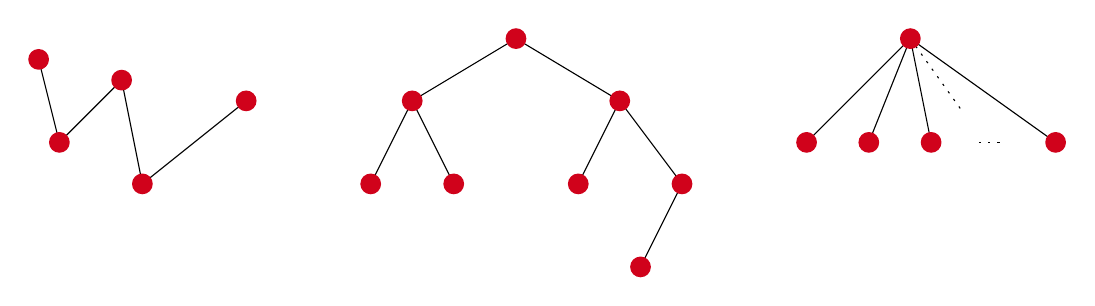
\begin{tikzpicture}[x=0.75pt,y=0.75pt,yscale=-1,xscale=1]
%uncomment if require: \path (0,193); %set diagram left start at 0, and has height of 193

%Straight Lines [id:da49703614339776037] 
\draw  [dash pattern={on 0.84pt off 2.51pt}]  (545,25) -- (570,60) ;
%Straight Lines [id:da8560002704789386] 
\draw    (545,25) -- (495,75) ;
%Straight Lines [id:da8111128726222414] 
\draw    (545,25) -- (525,75) ;
%Straight Lines [id:da706792274923423] 
\draw    (545,25) -- (555,75) ;
%Straight Lines [id:da46674031153499496] 
\draw    (545,25) -- (615,75) ;
%Straight Lines [id:da2902373414033316] 
\draw    (125,35) -- (135,75) ;
%Straight Lines [id:da9385080584462927] 
\draw    (135,75) -- (165,45) ;
%Straight Lines [id:da6001851670749982] 
\draw    (175,95) -- (165,45) ;
%Straight Lines [id:da6179902147981986] 
\draw    (175,95) -- (225,55) ;
%Shape: Circle [id:dp7325026650910265] 
\draw  [draw opacity=0][fill={rgb, 255:red, 208; green, 2; blue, 27 }  ,fill opacity=1 ] (120,35) .. controls (120,32.24) and (122.24,30) .. (125,30) .. controls (127.76,30) and (130,32.24) .. (130,35) .. controls (130,37.76) and (127.76,40) .. (125,40) .. controls (122.24,40) and (120,37.76) .. (120,35) -- cycle ;
%Shape: Circle [id:dp611790102044747] 
\draw  [draw opacity=0][fill={rgb, 255:red, 208; green, 2; blue, 27 }  ,fill opacity=1 ] (130,75) .. controls (130,72.24) and (132.24,70) .. (135,70) .. controls (137.76,70) and (140,72.24) .. (140,75) .. controls (140,77.76) and (137.76,80) .. (135,80) .. controls (132.24,80) and (130,77.76) .. (130,75) -- cycle ;
%Shape: Circle [id:dp3596636072841959] 
\draw  [draw opacity=0][fill={rgb, 255:red, 208; green, 2; blue, 27 }  ,fill opacity=1 ] (160,45) .. controls (160,42.24) and (162.24,40) .. (165,40) .. controls (167.76,40) and (170,42.24) .. (170,45) .. controls (170,47.76) and (167.76,50) .. (165,50) .. controls (162.24,50) and (160,47.76) .. (160,45) -- cycle ;
%Shape: Circle [id:dp7908891047683889] 
\draw  [draw opacity=0][fill={rgb, 255:red, 208; green, 2; blue, 27 }  ,fill opacity=1 ] (170,95) .. controls (170,92.24) and (172.24,90) .. (175,90) .. controls (177.76,90) and (180,92.24) .. (180,95) .. controls (180,97.76) and (177.76,100) .. (175,100) .. controls (172.24,100) and (170,97.76) .. (170,95) -- cycle ;
%Shape: Circle [id:dp5262181762220665] 
\draw  [draw opacity=0][fill={rgb, 255:red, 208; green, 2; blue, 27 }  ,fill opacity=1 ] (220,55) .. controls (220,52.24) and (222.24,50) .. (225,50) .. controls (227.76,50) and (230,52.24) .. (230,55) .. controls (230,57.76) and (227.76,60) .. (225,60) .. controls (222.24,60) and (220,57.76) .. (220,55) -- cycle ;
%Straight Lines [id:da006279841472952352] 
\draw    (355,25) -- (305,55) ;
%Straight Lines [id:da38151929511686866] 
\draw    (305,55) -- (285,95) ;
%Straight Lines [id:da8646233760724492] 
\draw    (305,55) -- (325,95) ;
%Straight Lines [id:da2659418830802085] 
\draw    (355,25) -- (405,55) ;
%Straight Lines [id:da9722511020037791] 
\draw    (405,55) -- (385,95) ;
%Straight Lines [id:da26948301296238975] 
\draw    (405,55) -- (435,95) ;
%Straight Lines [id:da12926477594492491] 
\draw    (435,95) -- (415,135) ;
%Shape: Circle [id:dp04492576400342452] 
\draw  [draw opacity=0][fill={rgb, 255:red, 208; green, 2; blue, 27 }  ,fill opacity=1 ] (400,55) .. controls (400,52.24) and (402.24,50) .. (405,50) .. controls (407.76,50) and (410,52.24) .. (410,55) .. controls (410,57.76) and (407.76,60) .. (405,60) .. controls (402.24,60) and (400,57.76) .. (400,55) -- cycle ;
%Shape: Circle [id:dp9515893329413634] 
\draw  [draw opacity=0][fill={rgb, 255:red, 208; green, 2; blue, 27 }  ,fill opacity=1 ] (350,25) .. controls (350,22.24) and (352.24,20) .. (355,20) .. controls (357.76,20) and (360,22.24) .. (360,25) .. controls (360,27.76) and (357.76,30) .. (355,30) .. controls (352.24,30) and (350,27.76) .. (350,25) -- cycle ;
%Shape: Circle [id:dp17095197522135586] 
\draw  [draw opacity=0][fill={rgb, 255:red, 208; green, 2; blue, 27 }  ,fill opacity=1 ] (300,55) .. controls (300,52.24) and (302.24,50) .. (305,50) .. controls (307.76,50) and (310,52.24) .. (310,55) .. controls (310,57.76) and (307.76,60) .. (305,60) .. controls (302.24,60) and (300,57.76) .. (300,55) -- cycle ;
%Shape: Circle [id:dp3002792957597066] 
\draw  [draw opacity=0][fill={rgb, 255:red, 208; green, 2; blue, 27 }  ,fill opacity=1 ] (280,95) .. controls (280,92.24) and (282.24,90) .. (285,90) .. controls (287.76,90) and (290,92.24) .. (290,95) .. controls (290,97.76) and (287.76,100) .. (285,100) .. controls (282.24,100) and (280,97.76) .. (280,95) -- cycle ;
%Shape: Circle [id:dp5407580206504065] 
\draw  [draw opacity=0][fill={rgb, 255:red, 208; green, 2; blue, 27 }  ,fill opacity=1 ] (320,95) .. controls (320,92.24) and (322.24,90) .. (325,90) .. controls (327.76,90) and (330,92.24) .. (330,95) .. controls (330,97.76) and (327.76,100) .. (325,100) .. controls (322.24,100) and (320,97.76) .. (320,95) -- cycle ;
%Shape: Circle [id:dp573748601669662] 
\draw  [draw opacity=0][fill={rgb, 255:red, 208; green, 2; blue, 27 }  ,fill opacity=1 ] (380,95) .. controls (380,92.24) and (382.24,90) .. (385,90) .. controls (387.76,90) and (390,92.24) .. (390,95) .. controls (390,97.76) and (387.76,100) .. (385,100) .. controls (382.24,100) and (380,97.76) .. (380,95) -- cycle ;
%Shape: Circle [id:dp3917663126214327] 
\draw  [draw opacity=0][fill={rgb, 255:red, 208; green, 2; blue, 27 }  ,fill opacity=1 ] (430,95) .. controls (430,92.24) and (432.24,90) .. (435,90) .. controls (437.76,90) and (440,92.24) .. (440,95) .. controls (440,97.76) and (437.76,100) .. (435,100) .. controls (432.24,100) and (430,97.76) .. (430,95) -- cycle ;
%Shape: Circle [id:dp5628588782173692] 
\draw  [draw opacity=0][fill={rgb, 255:red, 208; green, 2; blue, 27 }  ,fill opacity=1 ] (410,135) .. controls (410,132.24) and (412.24,130) .. (415,130) .. controls (417.76,130) and (420,132.24) .. (420,135) .. controls (420,137.76) and (417.76,140) .. (415,140) .. controls (412.24,140) and (410,137.76) .. (410,135) -- cycle ;
%Shape: Circle [id:dp8704892379172522] 
\draw  [draw opacity=0][fill={rgb, 255:red, 208; green, 2; blue, 27 }  ,fill opacity=1 ] (540,25) .. controls (540,22.24) and (542.24,20) .. (545,20) .. controls (547.76,20) and (550,22.24) .. (550,25) .. controls (550,27.76) and (547.76,30) .. (545,30) .. controls (542.24,30) and (540,27.76) .. (540,25) -- cycle ;
%Shape: Circle [id:dp922502556460108] 
\draw  [draw opacity=0][fill={rgb, 255:red, 208; green, 2; blue, 27 }  ,fill opacity=1 ] (490,75) .. controls (490,72.24) and (492.24,70) .. (495,70) .. controls (497.76,70) and (500,72.24) .. (500,75) .. controls (500,77.76) and (497.76,80) .. (495,80) .. controls (492.24,80) and (490,77.76) .. (490,75) -- cycle ;
%Shape: Circle [id:dp19932072180727434] 
\draw  [draw opacity=0][fill={rgb, 255:red, 208; green, 2; blue, 27 }  ,fill opacity=1 ] (520,75) .. controls (520,72.24) and (522.24,70) .. (525,70) .. controls (527.76,70) and (530,72.24) .. (530,75) .. controls (530,77.76) and (527.76,80) .. (525,80) .. controls (522.24,80) and (520,77.76) .. (520,75) -- cycle ;
%Shape: Circle [id:dp2630213009599035] 
\draw  [draw opacity=0][fill={rgb, 255:red, 208; green, 2; blue, 27 }  ,fill opacity=1 ] (550,75) .. controls (550,72.24) and (552.24,70) .. (555,70) .. controls (557.76,70) and (560,72.24) .. (560,75) .. controls (560,77.76) and (557.76,80) .. (555,80) .. controls (552.24,80) and (550,77.76) .. (550,75) -- cycle ;
%Shape: Circle [id:dp9778477086384065] 
\draw  [draw opacity=0][fill={rgb, 255:red, 208; green, 2; blue, 27 }  ,fill opacity=1 ] (610,75) .. controls (610,72.24) and (612.24,70) .. (615,70) .. controls (617.76,70) and (620,72.24) .. (620,75) .. controls (620,77.76) and (617.76,80) .. (615,80) .. controls (612.24,80) and (610,77.76) .. (610,75) -- cycle ;
%Straight Lines [id:da4037746415210903] 
\draw  [dash pattern={on 0.84pt off 2.51pt}]  (578,75) -- (590,75) ;




\end{tikzpicture}

	\end{center}
\end{example}



\begin{proposition}[Characterising Trees]
	The following are equivalent.
	\begin{enumerate}[label=(\alph*)]
		\item $G$ is a tree.
		\item $G$ is a maximal acyclic graph (adding any edge creates a cycle).
		\item $G$ is a minimal connected graph (removing any edge disconnects the graph).
	\end{enumerate}
\end{proposition}
\begin{proof}
	\emph{(a) $\implies$ (b)}. By definition $G$ is acyclic. Let $x, y \in V$ such that $xy \not \in E$. As $G$ is connected, there is an $xy$ path $P$. The that $xPy$ then defines a cycle.

	\emph{(b) $\implies$ (a)}. By definition $G$ is acyclic. 
	So for a contradiction assume $G$ is not connected and let $x, y$ be vertices from different components. Now note $G + xy$ is acyclic, but this contradicts the claim that $G$ is maximally acyclic.

	\emph{(a) $\implies$ (c)}. By definition $G$ is connected. Suppose, for a contradiction, that there exists some vertices $x, y \in E$ with $x \neq y$ and $G - xy$ is connected. But then there is some $xy$ path $P$ that does not use the edge $xy$, so $xPy$ is then a cycle, contradicting that $G$ is acyclic.

	\emph{(c) $\implies$ (a)}. By definition $G$ is connected. Again for a contradiction, assume that $G$ contains a cycle $C$. Then let $xy$ be an edge on $C$. We claim $G - xy$ is still connected. If $u, v \in V(G - xy)$ then let $P$ be a path in $G$ from $u$ to $v$. If $xy$ does not appear as consecutive vertices on this path, then $u$ is connected to $v$. Otherwise, we can consider a new path where we replace $x,y$ with the other vertices in $C - xy$ in order. Thus $u$ and $v$ are still connected. This contradicts the minimal connectedness of $G$. 

\end{proof}

\begin{definition}[Leaf]
	Let $G$ be a graph. A vertex $v \in V(G)$ is a \vocab{leaf} if $d(v) = 1$.
\end{definition}

For example, the tree below has three leaves.
\begin{center}
	

\tikzset{every picture/.style={line width=0.75pt}} %set default line width to 0.75pt        

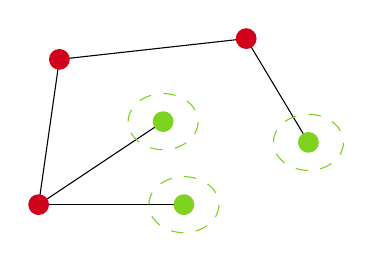
\begin{tikzpicture}[x=0.75pt,y=0.75pt,yscale=-1,xscale=1]
%uncomment if require: \path (0,193); %set diagram left start at 0, and has height of 193

%Straight Lines [id:da0984605927740948] 
\draw    (175,25) -- (165,95) ;
%Straight Lines [id:da6265757458636173] 
\draw    (165,95) -- (235,95) ;
%Straight Lines [id:da12182039563159297] 
\draw    (165,95) -- (225,55) ;
%Straight Lines [id:da667532625992501] 
\draw    (175,25) -- (265,15) ;
%Straight Lines [id:da4994952007175353] 
\draw    (265,15) -- (295,65) ;
%Shape: Circle [id:dp18461176684200264] 
\draw  [draw opacity=0][fill={rgb, 255:red, 208; green, 2; blue, 27 }  ,fill opacity=1 ] (170,25) .. controls (170,22.24) and (172.24,20) .. (175,20) .. controls (177.76,20) and (180,22.24) .. (180,25) .. controls (180,27.76) and (177.76,30) .. (175,30) .. controls (172.24,30) and (170,27.76) .. (170,25) -- cycle ;
%Shape: Circle [id:dp10060882656169834] 
\draw  [draw opacity=0][fill={rgb, 255:red, 208; green, 2; blue, 27 }  ,fill opacity=1 ] (160,95) .. controls (160,92.24) and (162.24,90) .. (165,90) .. controls (167.76,90) and (170,92.24) .. (170,95) .. controls (170,97.76) and (167.76,100) .. (165,100) .. controls (162.24,100) and (160,97.76) .. (160,95) -- cycle ;
%Shape: Circle [id:dp8035247431249818] 
\draw  [draw opacity=0][fill={rgb, 255:red, 208; green, 2; blue, 27 }  ,fill opacity=1 ] (260,15) .. controls (260,12.24) and (262.24,10) .. (265,10) .. controls (267.76,10) and (270,12.24) .. (270,15) .. controls (270,17.76) and (267.76,20) .. (265,20) .. controls (262.24,20) and (260,17.76) .. (260,15) -- cycle ;
%Shape: Circle [id:dp03884028492334557] 
\draw  [draw opacity=0][fill={rgb, 255:red, 126; green, 211; blue, 33 }  ,fill opacity=1 ] (220,55) .. controls (220,52.24) and (222.24,50) .. (225,50) .. controls (227.76,50) and (230,52.24) .. (230,55) .. controls (230,57.76) and (227.76,60) .. (225,60) .. controls (222.24,60) and (220,57.76) .. (220,55) -- cycle ;
%Shape: Circle [id:dp40784864189322] 
\draw  [draw opacity=0][fill={rgb, 255:red, 126; green, 211; blue, 33 }  ,fill opacity=1 ] (290,65) .. controls (290,62.24) and (292.24,60) .. (295,60) .. controls (297.76,60) and (300,62.24) .. (300,65) .. controls (300,67.76) and (297.76,70) .. (295,70) .. controls (292.24,70) and (290,67.76) .. (290,65) -- cycle ;
%Shape: Circle [id:dp034678543816174634] 
\draw  [draw opacity=0][fill={rgb, 255:red, 126; green, 211; blue, 33 }  ,fill opacity=1 ] (230,95) .. controls (230,92.24) and (232.24,90) .. (235,90) .. controls (237.76,90) and (240,92.24) .. (240,95) .. controls (240,97.76) and (237.76,100) .. (235,100) .. controls (232.24,100) and (230,97.76) .. (230,95) -- cycle ;
%Shape: Ellipse [id:dp47417663473871297] 
\draw  [color={rgb, 255:red, 126; green, 211; blue, 33 }  ,draw opacity=1 ][dash pattern={on 4.5pt off 4.5pt}] (208.13,55) .. controls (208.13,47.54) and (215.68,41.5) .. (225,41.5) .. controls (234.32,41.5) and (241.88,47.54) .. (241.88,55) .. controls (241.88,62.46) and (234.32,68.5) .. (225,68.5) .. controls (215.68,68.5) and (208.13,62.46) .. (208.13,55) -- cycle ;
%Shape: Ellipse [id:dp4680354598258094] 
\draw  [color={rgb, 255:red, 126; green, 211; blue, 33 }  ,draw opacity=1 ][dash pattern={on 4.5pt off 4.5pt}] (218.13,95) .. controls (218.13,87.54) and (225.68,81.5) .. (235,81.5) .. controls (244.32,81.5) and (251.88,87.54) .. (251.88,95) .. controls (251.88,102.46) and (244.32,108.5) .. (235,108.5) .. controls (225.68,108.5) and (218.13,102.46) .. (218.13,95) -- cycle ;
%Shape: Ellipse [id:dp7785817672164794] 
\draw  [color={rgb, 255:red, 126; green, 211; blue, 33 }  ,draw opacity=1 ][dash pattern={on 4.5pt off 4.5pt}] (278.13,65) .. controls (278.13,57.54) and (285.68,51.5) .. (295,51.5) .. controls (304.32,51.5) and (311.88,57.54) .. (311.88,65) .. controls (311.88,72.46) and (304.32,78.5) .. (295,78.5) .. controls (285.68,78.5) and (278.13,72.46) .. (278.13,65) -- cycle ;




\end{tikzpicture}

\end{center}
In general, trees has a leaf.

\begin{proposition}[Trees Have Leaves]
	Every tree $T$ with $|T| \geq 2$ has a leaf.
\end{proposition}
\begin{proof}
	Let $T$ be a tree with $|T| \geq 2$, and let $P$ be a path of maximum length in $T$, with $P = x_1 \dots x_k$. We claim that $d(x_k) = 1$. Observe that $\deg(x_k) \geq 1$, since $x_k x_{k - 1} \in E$. If $x_k$ is adjacent to another vertex $y \neq x_{k - 1}$, then either $y \in \{x_1, \dots, x_{k - 2}\}$, which would imply thar $T$ contains a cycle, or $y \not \in \{x_1, \dots, x_{k - 2}\}$, then $x_1 \dots x_k y$ is a path longer than $P$, which violates its maximality.
\end{proof}

\begin{remark}
	This proof gives us two leaves in $T$, which is the best we can hope for considering $P_n$ is a tree with exactly two leaves.
\end{remark}

\begin{proposition}[Edges of a Tree]
	Let $T$ be a tree. Then $e(T) = |T| - 1$.
\end{proposition}
\begin{proof}
	We will do induction on $n = |T|$. If $n = 1$, this is trivial as there is only one edge. Now given $T$ with at least 2 vertices, let $x$ be a leaf in $T$, and define $T' = T - x$.
	
	$T'$ must be acyclic, since we have only removed vertices. $T'$ must also be connected since for all $u, v \in V(T')$ there exists a path from $u$ to $v$ in $T$ that does not use $x$, so it is also a path from $u$ to $v$ in $T'$. Thus $T'$ is a tree.
	Thus by induction, $T'$ has $n - 2$ edges, and $e(T) = e(T') + 1 = |T| - 1$. 
\end{proof}

Now lets think about trees as subgraphs of other graphs.

\begin{definition}[Spanning Tree]
	Let $G$ be a graph. We say $T$ is a \vocab{spanning tree} of $G$ if $T$ is a tree on $V(G)$ and is a subgraph of $G$.
\end{definition}

\begin{center}
	

\tikzset{every picture/.style={line width=0.75pt}} %set default line width to 0.75pt        

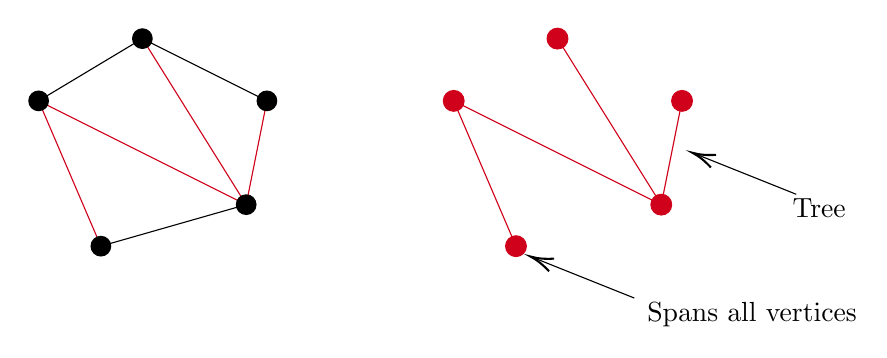
\begin{tikzpicture}[x=0.75pt,y=0.75pt,yscale=-1,xscale=1]
%uncomment if require: \path (0,193); %set diagram left start at 0, and has height of 193

%Straight Lines [id:da7720717972243504] 
\draw    (195,15) -- (145,45) ;
%Straight Lines [id:da7920300217957735] 
\draw [color={rgb, 255:red, 208; green, 2; blue, 27 }  ,draw opacity=1 ]   (175,115) -- (145,45) ;
%Straight Lines [id:da20392691285127829] 
\draw    (175,115) -- (245,95) ;
%Straight Lines [id:da8350342542026185] 
\draw [color={rgb, 255:red, 208; green, 2; blue, 27 }  ,draw opacity=1 ]   (245,95) -- (255,45) ;
%Straight Lines [id:da9158971334401541] 
\draw    (195,15) -- (255,45) ;
%Straight Lines [id:da18144577006731655] 
\draw [color={rgb, 255:red, 208; green, 2; blue, 27 }  ,draw opacity=1 ]   (195,15) -- (245,95) ;
%Straight Lines [id:da7793007821979472] 
\draw [color={rgb, 255:red, 208; green, 2; blue, 27 }  ,draw opacity=1 ]   (145,45) -- (245,95) ;
%Shape: Circle [id:dp1682506259527774] 
\draw  [draw opacity=0][fill={rgb, 255:red, 0; green, 0; blue, 0 }  ,fill opacity=1 ] (190,15) .. controls (190,12.24) and (192.24,10) .. (195,10) .. controls (197.76,10) and (200,12.24) .. (200,15) .. controls (200,17.76) and (197.76,20) .. (195,20) .. controls (192.24,20) and (190,17.76) .. (190,15) -- cycle ;
%Shape: Circle [id:dp6060797868745955] 
\draw  [draw opacity=0][fill={rgb, 255:red, 0; green, 0; blue, 0 }  ,fill opacity=1 ] (140,45) .. controls (140,42.24) and (142.24,40) .. (145,40) .. controls (147.76,40) and (150,42.24) .. (150,45) .. controls (150,47.76) and (147.76,50) .. (145,50) .. controls (142.24,50) and (140,47.76) .. (140,45) -- cycle ;
%Shape: Circle [id:dp5532360644089358] 
\draw  [draw opacity=0][fill={rgb, 255:red, 0; green, 0; blue, 0 }  ,fill opacity=1 ] (170,115) .. controls (170,112.24) and (172.24,110) .. (175,110) .. controls (177.76,110) and (180,112.24) .. (180,115) .. controls (180,117.76) and (177.76,120) .. (175,120) .. controls (172.24,120) and (170,117.76) .. (170,115) -- cycle ;
%Shape: Circle [id:dp9976784820641885] 
\draw  [draw opacity=0][fill={rgb, 255:red, 0; green, 0; blue, 0 }  ,fill opacity=1 ] (240,95) .. controls (240,92.24) and (242.24,90) .. (245,90) .. controls (247.76,90) and (250,92.24) .. (250,95) .. controls (250,97.76) and (247.76,100) .. (245,100) .. controls (242.24,100) and (240,97.76) .. (240,95) -- cycle ;
%Shape: Circle [id:dp362434366455488] 
\draw  [draw opacity=0][fill={rgb, 255:red, 0; green, 0; blue, 0 }  ,fill opacity=1 ] (250,45) .. controls (250,42.24) and (252.24,40) .. (255,40) .. controls (257.76,40) and (260,42.24) .. (260,45) .. controls (260,47.76) and (257.76,50) .. (255,50) .. controls (252.24,50) and (250,47.76) .. (250,45) -- cycle ;
%Straight Lines [id:da15805292190155373] 
\draw [color={rgb, 255:red, 208; green, 2; blue, 27 }  ,draw opacity=1 ][fill={rgb, 255:red, 208; green, 2; blue, 27 }  ,fill opacity=1 ]   (375,115) -- (345,45) ;
%Straight Lines [id:da8535130805001211] 
\draw [color={rgb, 255:red, 208; green, 2; blue, 27 }  ,draw opacity=1 ][fill={rgb, 255:red, 208; green, 2; blue, 27 }  ,fill opacity=1 ]   (445,95) -- (455,45) ;
%Straight Lines [id:da8314095713427262] 
\draw [color={rgb, 255:red, 208; green, 2; blue, 27 }  ,draw opacity=1 ][fill={rgb, 255:red, 208; green, 2; blue, 27 }  ,fill opacity=1 ]   (395,15) -- (445,95) ;
%Straight Lines [id:da7752162474752384] 
\draw [color={rgb, 255:red, 208; green, 2; blue, 27 }  ,draw opacity=1 ][fill={rgb, 255:red, 208; green, 2; blue, 27 }  ,fill opacity=1 ]   (345,45) -- (445,95) ;
%Shape: Circle [id:dp9210808159738209] 
\draw  [color={rgb, 255:red, 208; green, 2; blue, 27 }  ,draw opacity=1 ][fill={rgb, 255:red, 208; green, 2; blue, 27 }  ,fill opacity=1 ] (390,15) .. controls (390,12.24) and (392.24,10) .. (395,10) .. controls (397.76,10) and (400,12.24) .. (400,15) .. controls (400,17.76) and (397.76,20) .. (395,20) .. controls (392.24,20) and (390,17.76) .. (390,15) -- cycle ;
%Shape: Circle [id:dp3107879115086415] 
\draw  [color={rgb, 255:red, 208; green, 2; blue, 27 }  ,draw opacity=1 ][fill={rgb, 255:red, 208; green, 2; blue, 27 }  ,fill opacity=1 ] (340,45) .. controls (340,42.24) and (342.24,40) .. (345,40) .. controls (347.76,40) and (350,42.24) .. (350,45) .. controls (350,47.76) and (347.76,50) .. (345,50) .. controls (342.24,50) and (340,47.76) .. (340,45) -- cycle ;
%Shape: Circle [id:dp6855923108139758] 
\draw  [color={rgb, 255:red, 208; green, 2; blue, 27 }  ,draw opacity=1 ][fill={rgb, 255:red, 208; green, 2; blue, 27 }  ,fill opacity=1 ] (370,115) .. controls (370,112.24) and (372.24,110) .. (375,110) .. controls (377.76,110) and (380,112.24) .. (380,115) .. controls (380,117.76) and (377.76,120) .. (375,120) .. controls (372.24,120) and (370,117.76) .. (370,115) -- cycle ;
%Shape: Circle [id:dp7351941658035576] 
\draw  [color={rgb, 255:red, 208; green, 2; blue, 27 }  ,draw opacity=1 ][fill={rgb, 255:red, 208; green, 2; blue, 27 }  ,fill opacity=1 ] (440,95) .. controls (440,92.24) and (442.24,90) .. (445,90) .. controls (447.76,90) and (450,92.24) .. (450,95) .. controls (450,97.76) and (447.76,100) .. (445,100) .. controls (442.24,100) and (440,97.76) .. (440,95) -- cycle ;
%Shape: Circle [id:dp33930610746251866] 
\draw  [color={rgb, 255:red, 208; green, 2; blue, 27 }  ,draw opacity=1 ][fill={rgb, 255:red, 208; green, 2; blue, 27 }  ,fill opacity=1 ] (450,45) .. controls (450,42.24) and (452.24,40) .. (455,40) .. controls (457.76,40) and (460,42.24) .. (460,45) .. controls (460,47.76) and (457.76,50) .. (455,50) .. controls (452.24,50) and (450,47.76) .. (450,45) -- cycle ;
%Straight Lines [id:da6794496736217942] 
\draw    (510,90) -- (461.86,70.74) ;
\draw [shift={(460,70)}, rotate = 381.8] [color={rgb, 255:red, 0; green, 0; blue, 0 }  ][line width=0.75]    (10.93,-3.29) .. controls (6.95,-1.4) and (3.31,-0.3) .. (0,0) .. controls (3.31,0.3) and (6.95,1.4) .. (10.93,3.29)   ;
%Straight Lines [id:da24613239577970836] 
\draw    (432,140) -- (383.86,120.74) ;
\draw [shift={(382,120)}, rotate = 381.8] [color={rgb, 255:red, 0; green, 0; blue, 0 }  ][line width=0.75]    (10.93,-3.29) .. controls (6.95,-1.4) and (3.31,-0.3) .. (0,0) .. controls (3.31,0.3) and (6.95,1.4) .. (10.93,3.29)   ;

% Text Node
\draw (507,91) node [anchor=north west][inner sep=0.75pt]   [align=left] {Tree};
% Text Node
\draw (437,141) node [anchor=north west][inner sep=0.75pt]   [align=left] {Spans all vertices};


\end{tikzpicture}

\end{center}

Spanning trees are useful in a number of contexts, one of which is giving a sensible ordering to the vertices of a graph. They are particularly useful because of the following result.

\begin{proposition}[Connected Graphs have Spanning Trees]
	Every connected graph contains a spanning tree.
\end{proposition}
\begin{proof}
	A tree is a minimal connected graph. So take the connected graph and remove edges until it becomes a minimal connected graph. Then this will be a subgraph of the original graph, and will thus be a spanning tree.
\end{proof}

\section{Bipartite Graphs}

The next type of graph we will look at is \emph{bipartite} graphs.

\begin{definition}[Bipartite Graphs]
	A graph $G = (V, E)$ is \vocab{bipartite} if $V = A \cup B$ where $A \cap B = \emptyset$ and all edges $xy \in E$ have either $x \in A, y \in B$ or $x \in B, y \in A$.
\end{definition}

\begin{example}[Example of Bipartite Graphs]
	The graph below is bipartite, with vertices in the set $A$ being coloured red and vertices in the set $B$ being coloured blue.
	\begin{center}
		

\tikzset{every picture/.style={line width=0.75pt}} %set default line width to 0.75pt        

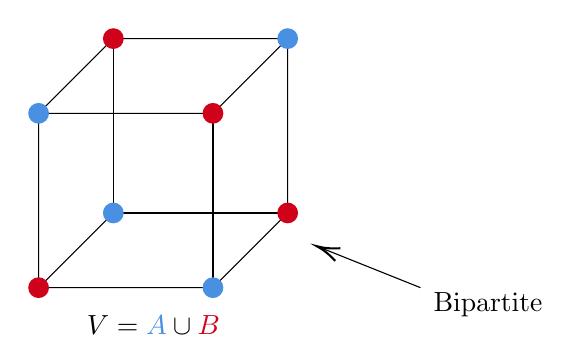
\begin{tikzpicture}[x=0.75pt,y=0.75pt,yscale=-1,xscale=1]
%uncomment if require: \path (0,193); %set diagram left start at 0, and has height of 193

%Straight Lines [id:da6060270401424458] 
\draw    (216,40) -- (216,124) ;
%Straight Lines [id:da23724217319822305] 
\draw    (300,124) -- (216,124) ;
%Straight Lines [id:da19809780044648873] 
\draw    (180,160) -- (216,124) ;
%Straight Lines [id:da24613239577970836] 
\draw    (364,160) -- (315.86,140.74) ;
\draw [shift={(314,140)}, rotate = 381.8] [color={rgb, 255:red, 0; green, 0; blue, 0 }  ][line width=0.75]    (10.93,-3.29) .. controls (6.95,-1.4) and (3.31,-0.3) .. (0,0) .. controls (3.31,0.3) and (6.95,1.4) .. (10.93,3.29)   ;
%Shape: Cube [id:dp9216272317281227] 
\draw   (180,76) -- (216,40) -- (300,40) -- (300,124) -- (264,160) -- (180,160) -- cycle ; \draw   (300,40) -- (264,76) -- (180,76) ; \draw   (264,76) -- (264,160) ;
%Shape: Circle [id:dp7313331826223877] 
\draw  [draw opacity=0][fill={rgb, 255:red, 208; green, 2; blue, 27 }  ,fill opacity=1 ] (175,160) .. controls (175,157.24) and (177.24,155) .. (180,155) .. controls (182.76,155) and (185,157.24) .. (185,160) .. controls (185,162.76) and (182.76,165) .. (180,165) .. controls (177.24,165) and (175,162.76) .. (175,160) -- cycle ;
%Shape: Circle [id:dp9469737817920821] 
\draw  [draw opacity=0][fill={rgb, 255:red, 74; green, 144; blue, 226 }  ,fill opacity=1 ] (259,160) .. controls (259,157.24) and (261.24,155) .. (264,155) .. controls (266.76,155) and (269,157.24) .. (269,160) .. controls (269,162.76) and (266.76,165) .. (264,165) .. controls (261.24,165) and (259,162.76) .. (259,160) -- cycle ;
%Shape: Circle [id:dp927144427433717] 
\draw  [draw opacity=0][fill={rgb, 255:red, 208; green, 2; blue, 27 }  ,fill opacity=1 ] (295,124) .. controls (295,121.24) and (297.24,119) .. (300,119) .. controls (302.76,119) and (305,121.24) .. (305,124) .. controls (305,126.76) and (302.76,129) .. (300,129) .. controls (297.24,129) and (295,126.76) .. (295,124) -- cycle ;
%Shape: Circle [id:dp6195253711881875] 
\draw  [draw opacity=0][fill={rgb, 255:red, 74; green, 144; blue, 226 }  ,fill opacity=1 ] (295,40) .. controls (295,37.24) and (297.24,35) .. (300,35) .. controls (302.76,35) and (305,37.24) .. (305,40) .. controls (305,42.76) and (302.76,45) .. (300,45) .. controls (297.24,45) and (295,42.76) .. (295,40) -- cycle ;
%Shape: Circle [id:dp5745873981618578] 
\draw  [draw opacity=0][fill={rgb, 255:red, 208; green, 2; blue, 27 }  ,fill opacity=1 ] (259,76) .. controls (259,73.24) and (261.24,71) .. (264,71) .. controls (266.76,71) and (269,73.24) .. (269,76) .. controls (269,78.76) and (266.76,81) .. (264,81) .. controls (261.24,81) and (259,78.76) .. (259,76) -- cycle ;
%Shape: Circle [id:dp0848509986260515] 
\draw  [draw opacity=0][fill={rgb, 255:red, 74; green, 144; blue, 226 }  ,fill opacity=1 ] (175,76) .. controls (175,73.24) and (177.24,71) .. (180,71) .. controls (182.76,71) and (185,73.24) .. (185,76) .. controls (185,78.76) and (182.76,81) .. (180,81) .. controls (177.24,81) and (175,78.76) .. (175,76) -- cycle ;
%Shape: Circle [id:dp5237597618279684] 
\draw  [draw opacity=0][fill={rgb, 255:red, 208; green, 2; blue, 27 }  ,fill opacity=1 ] (211,40) .. controls (211,37.24) and (213.24,35) .. (216,35) .. controls (218.76,35) and (221,37.24) .. (221,40) .. controls (221,42.76) and (218.76,45) .. (216,45) .. controls (213.24,45) and (211,42.76) .. (211,40) -- cycle ;
%Shape: Circle [id:dp7456524979791003] 
\draw  [draw opacity=0][fill={rgb, 255:red, 74; green, 144; blue, 226 }  ,fill opacity=1 ] (211,124) .. controls (211,121.24) and (213.24,119) .. (216,119) .. controls (218.76,119) and (221,121.24) .. (221,124) .. controls (221,126.76) and (218.76,129) .. (216,129) .. controls (213.24,129) and (211,126.76) .. (211,124) -- cycle ;

% Text Node
\draw (369,161) node [anchor=north west][inner sep=0.75pt]   [align=left] {Bipartite};
% Text Node
\draw (202,172) node [anchor=north west][inner sep=0.75pt]    {$V=\textcolor[rgb]{0.29,0.56,0.89}{A} \cup \textcolor[rgb]{0.82,0.01,0.11}{B}$};


\end{tikzpicture}

	\end{center}

	An example of a non-bipartite graph is $C_5$. To see this, we can start by choosing a vertex to be in $A$ (without loss of generality), then the adjacent vertices must be in $B$, but then their adjacent vertices must be in $A$, but then there is an edge between two vertices in $A$. This is shown below.

	\begin{center}
		

\tikzset{every picture/.style={line width=0.75pt}} %set default line width to 0.75pt        

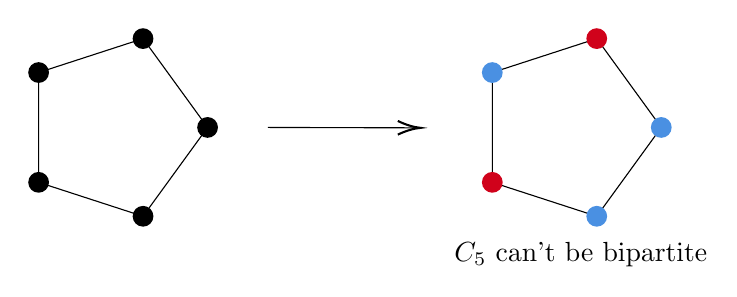
\begin{tikzpicture}[x=0.75pt,y=0.75pt,yscale=-1,xscale=1]
%uncomment if require: \path (0,193); %set diagram left start at 0, and has height of 193

%Shape: Regular Polygon [id:dp6479462597087118] 
\draw   (206.41,87.8) -- (175.31,130.6) -- (125,114.25) -- (125,61.35) -- (175.31,45) -- cycle ;
%Shape: Circle [id:dp9268028209058927] 
\draw  [draw opacity=0][fill={rgb, 255:red, 0; green, 0; blue, 0 }  ,fill opacity=1 ] (201.41,87.8) .. controls (201.41,85.04) and (203.64,82.8) .. (206.41,82.8) .. controls (209.17,82.8) and (211.41,85.04) .. (211.41,87.8) .. controls (211.41,90.56) and (209.17,92.8) .. (206.41,92.8) .. controls (203.64,92.8) and (201.41,90.56) .. (201.41,87.8) -- cycle ;
%Shape: Circle [id:dp5164482643400302] 
\draw  [draw opacity=0][fill={rgb, 255:red, 0; green, 0; blue, 0 }  ,fill opacity=1 ] (170.31,45) .. controls (170.31,42.24) and (172.55,40) .. (175.31,40) .. controls (178.07,40) and (180.31,42.24) .. (180.31,45) .. controls (180.31,47.76) and (178.07,50) .. (175.31,50) .. controls (172.55,50) and (170.31,47.76) .. (170.31,45) -- cycle ;
%Shape: Circle [id:dp6340446217566587] 
\draw  [draw opacity=0][fill={rgb, 255:red, 0; green, 0; blue, 0 }  ,fill opacity=1 ] (120,61.35) .. controls (120,58.59) and (122.24,56.35) .. (125,56.35) .. controls (127.76,56.35) and (130,58.59) .. (130,61.35) .. controls (130,64.11) and (127.76,66.35) .. (125,66.35) .. controls (122.24,66.35) and (120,64.11) .. (120,61.35) -- cycle ;
%Shape: Circle [id:dp6354510885840486] 
\draw  [draw opacity=0][fill={rgb, 255:red, 0; green, 0; blue, 0 }  ,fill opacity=1 ] (120,114.25) .. controls (120,111.49) and (122.24,109.25) .. (125,109.25) .. controls (127.76,109.25) and (130,111.49) .. (130,114.25) .. controls (130,117.01) and (127.76,119.25) .. (125,119.25) .. controls (122.24,119.25) and (120,117.01) .. (120,114.25) -- cycle ;
%Shape: Circle [id:dp7177331645001392] 
\draw  [draw opacity=0][fill={rgb, 255:red, 0; green, 0; blue, 0 }  ,fill opacity=1 ] (170.31,130.6) .. controls (170.31,127.83) and (172.55,125.6) .. (175.31,125.6) .. controls (178.07,125.6) and (180.31,127.83) .. (180.31,130.6) .. controls (180.31,133.36) and (178.07,135.6) .. (175.31,135.6) .. controls (172.55,135.6) and (170.31,133.36) .. (170.31,130.6) -- cycle ;
%Straight Lines [id:da044616960583838905] 
\draw    (235.41,87.8) -- (307,87.99) ;
\draw [shift={(309,88)}, rotate = 180.16] [color={rgb, 255:red, 0; green, 0; blue, 0 }  ][line width=0.75]    (10.93,-3.29) .. controls (6.95,-1.4) and (3.31,-0.3) .. (0,0) .. controls (3.31,0.3) and (6.95,1.4) .. (10.93,3.29)   ;
%Shape: Regular Polygon [id:dp6720141486992529] 
\draw   (425,87.8) -- (393.91,130.6) -- (343.59,114.25) -- (343.59,61.35) -- (393.91,45) -- cycle ;
%Shape: Circle [id:dp6878881253571169] 
\draw  [draw opacity=0][fill={rgb, 255:red, 74; green, 144; blue, 226 }  ,fill opacity=1 ] (420,87.8) .. controls (420,85.04) and (422.24,82.8) .. (425,82.8) .. controls (427.76,82.8) and (430,85.04) .. (430,87.8) .. controls (430,90.56) and (427.76,92.8) .. (425,92.8) .. controls (422.24,92.8) and (420,90.56) .. (420,87.8) -- cycle ;
%Shape: Circle [id:dp7845528979637783] 
\draw  [draw opacity=0][fill={rgb, 255:red, 208; green, 2; blue, 27 }  ,fill opacity=1 ] (388.91,45) .. controls (388.91,42.24) and (391.14,40) .. (393.91,40) .. controls (396.67,40) and (398.91,42.24) .. (398.91,45) .. controls (398.91,47.76) and (396.67,50) .. (393.91,50) .. controls (391.14,50) and (388.91,47.76) .. (388.91,45) -- cycle ;
%Shape: Circle [id:dp35893358645915385] 
\draw  [draw opacity=0][fill={rgb, 255:red, 74; green, 144; blue, 226 }  ,fill opacity=1 ] (338.59,61.35) .. controls (338.59,58.59) and (340.83,56.35) .. (343.59,56.35) .. controls (346.36,56.35) and (348.59,58.59) .. (348.59,61.35) .. controls (348.59,64.11) and (346.36,66.35) .. (343.59,66.35) .. controls (340.83,66.35) and (338.59,64.11) .. (338.59,61.35) -- cycle ;
%Shape: Circle [id:dp814616877870825] 
\draw  [draw opacity=0][fill={rgb, 255:red, 208; green, 2; blue, 27 }  ,fill opacity=1 ] (338.59,114.25) .. controls (338.59,111.49) and (340.83,109.25) .. (343.59,109.25) .. controls (346.36,109.25) and (348.59,111.49) .. (348.59,114.25) .. controls (348.59,117.01) and (346.36,119.25) .. (343.59,119.25) .. controls (340.83,119.25) and (338.59,117.01) .. (338.59,114.25) -- cycle ;
%Shape: Circle [id:dp9973985318086398] 
\draw  [draw opacity=0][fill={rgb, 255:red, 74; green, 144; blue, 226 }  ,fill opacity=1 ] (388.91,130.6) .. controls (388.91,127.83) and (391.14,125.6) .. (393.91,125.6) .. controls (396.67,125.6) and (398.91,127.83) .. (398.91,130.6) .. controls (398.91,133.36) and (396.67,135.6) .. (393.91,135.6) .. controls (391.14,135.6) and (388.91,133.36) .. (388.91,130.6) -- cycle ;

% Text Node
\draw (324,142) node [anchor=north west][inner sep=0.75pt]   [align=left] {$\displaystyle C_{5}$ can't be bipartite};


\end{tikzpicture}

	\end{center}

\end{example}

The argument given for $C_5$ works in general.

\begin{proposition}[Bipartite Cyclic Graphs]
	The cycle $C_{2k + 1}$ is \emph{not} bipartite, and the cycle $C_{2k}$ \emph{is} bipartite.
\end{proposition}
\begin{proof}
	Assume that $C_{2k + 1}$ is bipartite. Then there must be disjoint sets $A$ and $B$, and as $2k + 1$ is odd, we must have (without loss of generality), $|A| > |B|$. Now let's count the edges between $A$ and $B$. This must be $2|A|$ and also $2|B|$, as every vertex has degree 2. But then $|A| = |B|$, which is a contradiction.

	For $C_{2n}$, we can let $v_i \in A$ if $i$ is even and $v_i \in B$ if $i$ is odd. Then a vertex $i$ only has edges to vertices $i - 1$ and $i + 1 \pmod{2}$, which have opposite parity. Thus all edges are between $A$ and $B$, as required.
\end{proof}

There is then a natural question: given some arbitrary graph $G$, how do we determine if a given graph is bipartite? It turns out that there is a nice check for `bipartness'. We will state the result and then do some setup before we prove it. 

\begin{proposition}[Bipartite Criterion]
	A graph $G$ is bipartite if and only if $G$ contains no odd cycles.
\end{proposition}

We need to first develop some theory regarding \emph{circuits}.
Informally, a circuit is like a cycle where we can revisit vertices.


\begin{definition}[Circuit]
A circuit is a sequence $x_1 \dots x_l$ where $x_1 = x_l$ and $x_i x_{i + 1} \in E$. The \vocab{length} of the circuit is $l - 1$, the number of edges traversed in the circuit.
\end{definition}

\begin{definition}[Odd Circuits]
	If the length of a circuit is odd, then we say it is an \vocab{odd circuit}.
\end{definition}

\begin{proposition}
An odd circuit contains an odd cycle.	
\end{proposition}
\begin{proof}
	We will prove this by induction on the length of the circuit. For a circuit of length $3$, the circuit must be a cycle.
	In general, let $C = x_1 \dots x_l$ be our circuit. If $x_1, \dots, x_{l - 1}$ are distinct, then $C$ is a cycle and we are done. 
	
	Otherwise, there exists some $z \in C$ that is repeated. We write 
	$$C = x_1 \dots x_a z x_{a + 2} \dots x_{b} z x_{b + 2} \dots x_l.$$
	We define $C' = x_1 \dots x_a z x_{b + 2} \dots x_l$ and $C'' = z x_{a + 2} \dots x_b z$. The length of $C'$ and $C''$ is strictly less than the length of $C$. One of these circuits must have odd length, and by induction that odd circuit contains an odd cycle.
\end{proof}

We can now prove our original bipartness criterion, that a graph is bipartite if and only if it contains no odd cycles.

\begin{proof}[Proof (Bipartite Criterion)]
	If $G$ was bipartite and contained an odd cycle, then there exists an odd cycle that is bipartite. But this is a contradiction.

	Now if $G$ is not bipartite, we can induct on the number of vertices. For $|G| = 1$, this holds. Now if $G$ is not connected, let $C_1, \dots, C_k$ be the components of $G$. We may now apply our induction to each component of $G$ to obtain a bipartitian $V(C_i) = A_i \cup B_i$ for each $i \in 1, \dots, k$. Then $A = A_1 \cup \dots A_k$ and $B = B_1 \cup B_k$ is a bipartitian for the whole graph. 
	
	We may now assume without loss of generality that $G$ is connected. Fix some vertex $v \in V$, and define 
	\begin{align*}
		A &= \{u \in V \mid d(u, v) \text{ is odd} \} \\
		B &=  \{u \in V \mid d(u, v) \text{ is even} \}
	\end{align*}
	We claim that $A \cup B$ is a bipartitian.

	Assume (for a contradiction) that $u_1$ is adjacent to $u_2$ and $d(u_1, v) \cong d(u_2, v) \pmod{2}$. Then there exists paths $P_1$ from $v$ to $u_1$ and $P_2$ from $u_2$ to $v$ with $|P_1| \equiv |P_2|$. But this implies that $vP_1u_1 u_2 P_2$ defines a odd circuit in $G$. Therefore, by our previous proposition, $G$ contains an odd cycle, which is a contradiction. 
\end{proof}
% Looking back at $k$-regular graphs, we are going to introduce some definitions.

\chapter{Hall's Theorem}

In this chapter, we will build up our knowledge of \emph{matchings} so that we can prove the first theorem of the course -- Hall's theorem.

\section{Matchings}

An appropriate place to start is probably by defining what a matching is.

\begin{definition}[Matching]
	A \vocab{matching} of $G$ is a collection of edges $M \subseteq E$ so that $\forall e_1, e_2 \in M$ with $e_1 \neq e_2$ has $e_1 \cap e_2 = \emptyset$.
\end{definition}

\begin{center}
	

\tikzset{every picture/.style={line width=0.75pt}} %set default line width to 0.75pt        

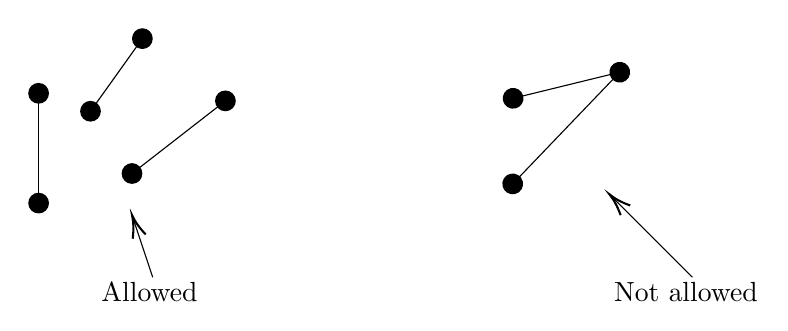
\begin{tikzpicture}[x=0.75pt,y=0.75pt,yscale=-1,xscale=1]
%uncomment if require: \path (0,193); %set diagram left start at 0, and has height of 193

%Shape: Circle [id:dp6340446217566587] 
\draw  [draw opacity=0][fill={rgb, 255:red, 0; green, 0; blue, 0 }  ,fill opacity=1 ] (120,61.35) .. controls (120,58.59) and (122.24,56.35) .. (125,56.35) .. controls (127.76,56.35) and (130,58.59) .. (130,61.35) .. controls (130,64.11) and (127.76,66.35) .. (125,66.35) .. controls (122.24,66.35) and (120,64.11) .. (120,61.35) -- cycle ;
%Shape: Circle [id:dp6354510885840486] 
\draw  [draw opacity=0][fill={rgb, 255:red, 0; green, 0; blue, 0 }  ,fill opacity=1 ] (120,114.25) .. controls (120,111.49) and (122.24,109.25) .. (125,109.25) .. controls (127.76,109.25) and (130,111.49) .. (130,114.25) .. controls (130,117.01) and (127.76,119.25) .. (125,119.25) .. controls (122.24,119.25) and (120,117.01) .. (120,114.25) -- cycle ;
%Straight Lines [id:da9660545408645501] 
\draw    (125,61.35) -- (125,114.25) ;
%Shape: Circle [id:dp07371359600393312] 
\draw  [draw opacity=0][fill={rgb, 255:red, 0; green, 0; blue, 0 }  ,fill opacity=1 ] (170,35) .. controls (170,32.24) and (172.24,30) .. (175,30) .. controls (177.76,30) and (180,32.24) .. (180,35) .. controls (180,37.76) and (177.76,40) .. (175,40) .. controls (172.24,40) and (170,37.76) .. (170,35) -- cycle ;
%Shape: Circle [id:dp7298704478232834] 
\draw  [draw opacity=0][fill={rgb, 255:red, 0; green, 0; blue, 0 }  ,fill opacity=1 ] (145,70) .. controls (145,67.24) and (147.24,65) .. (150,65) .. controls (152.76,65) and (155,67.24) .. (155,70) .. controls (155,72.76) and (152.76,75) .. (150,75) .. controls (147.24,75) and (145,72.76) .. (145,70) -- cycle ;
%Straight Lines [id:da7189218910738701] 
\draw    (175,35) -- (150,70) ;
%Shape: Circle [id:dp2883327905774512] 
\draw  [draw opacity=0][fill={rgb, 255:red, 0; green, 0; blue, 0 }  ,fill opacity=1 ] (165,100) .. controls (165,97.24) and (167.24,95) .. (170,95) .. controls (172.76,95) and (175,97.24) .. (175,100) .. controls (175,102.76) and (172.76,105) .. (170,105) .. controls (167.24,105) and (165,102.76) .. (165,100) -- cycle ;
%Shape: Circle [id:dp895782424476154] 
\draw  [draw opacity=0][fill={rgb, 255:red, 0; green, 0; blue, 0 }  ,fill opacity=1 ] (210,65) .. controls (210,62.24) and (212.24,60) .. (215,60) .. controls (217.76,60) and (220,62.24) .. (220,65) .. controls (220,67.76) and (217.76,70) .. (215,70) .. controls (212.24,70) and (210,67.76) .. (210,65) -- cycle ;
%Straight Lines [id:da41020563458187653] 
\draw    (170,100) -- (215,65) ;
%Shape: Circle [id:dp3162158662674279] 
\draw  [draw opacity=0][fill={rgb, 255:red, 0; green, 0; blue, 0 }  ,fill opacity=1 ] (403.81,46.34) .. controls (406.49,45.68) and (409.2,47.32) .. (409.86,50.01) .. controls (410.51,52.69) and (408.87,55.39) .. (406.19,56.05) .. controls (403.5,56.71) and (400.8,55.07) .. (400.14,52.38) .. controls (399.49,49.7) and (401.13,46.99) .. (403.81,46.34) -- cycle ;
%Shape: Circle [id:dp9128286694228138] 
\draw  [draw opacity=0][fill={rgb, 255:red, 0; green, 0; blue, 0 }  ,fill opacity=1 ] (352.43,58.91) .. controls (355.11,58.26) and (357.81,59.9) .. (358.47,62.58) .. controls (359.13,65.26) and (357.48,67.97) .. (354.8,68.63) .. controls (352.12,69.28) and (349.41,67.64) .. (348.76,64.96) .. controls (348.1,62.27) and (349.74,59.57) .. (352.43,58.91) -- cycle ;
%Straight Lines [id:da7665473567986095] 
\draw    (405,51.19) -- (353.61,63.77) ;
%Shape: Circle [id:dp3935047864716522] 
\draw  [draw opacity=0][fill={rgb, 255:red, 0; green, 0; blue, 0 }  ,fill opacity=1 ] (352.22,100.14) .. controls (354.9,99.49) and (357.61,101.13) .. (358.26,103.81) .. controls (358.92,106.49) and (357.28,109.2) .. (354.6,109.86) .. controls (351.91,110.51) and (349.21,108.87) .. (348.55,106.19) .. controls (347.9,103.5) and (349.54,100.8) .. (352.22,100.14) -- cycle ;
%Straight Lines [id:da4625514392127944] 
\draw    (405,51.19) -- (353.41,105) ;
%Straight Lines [id:da12607406579399916] 
\draw    (180,150) -- (170.63,121.9) ;
\draw [shift={(170,120)}, rotate = 431.57] [color={rgb, 255:red, 0; green, 0; blue, 0 }  ][line width=0.75]    (10.93,-3.29) .. controls (6.95,-1.4) and (3.31,-0.3) .. (0,0) .. controls (3.31,0.3) and (6.95,1.4) .. (10.93,3.29)   ;
%Straight Lines [id:da3703285294357822] 
\draw    (440,150) -- (401.41,111.41) ;
\draw [shift={(400,110)}, rotate = 405] [color={rgb, 255:red, 0; green, 0; blue, 0 }  ][line width=0.75]    (10.93,-3.29) .. controls (6.95,-1.4) and (3.31,-0.3) .. (0,0) .. controls (3.31,0.3) and (6.95,1.4) .. (10.93,3.29)   ;

% Text Node
\draw (154,151) node [anchor=north west][inner sep=0.75pt]   [align=left] {Allowed};
% Text Node
\draw (401,151) node [anchor=north west][inner sep=0.75pt]   [align=left] {Not allowed};


\end{tikzpicture}

\end{center}

\begin{definition}[Saturated]
	Given a graph $G = (V, E)$ and a matching $M$ in $G$, we say that a vertex $v \in V$ is \vocab{saturated by $M$} if there exists an edge in $M$ containing $v$. 
\end{definition}

\begin{center}
	

\tikzset{every picture/.style={line width=0.75pt}} %set default line width to 0.75pt        

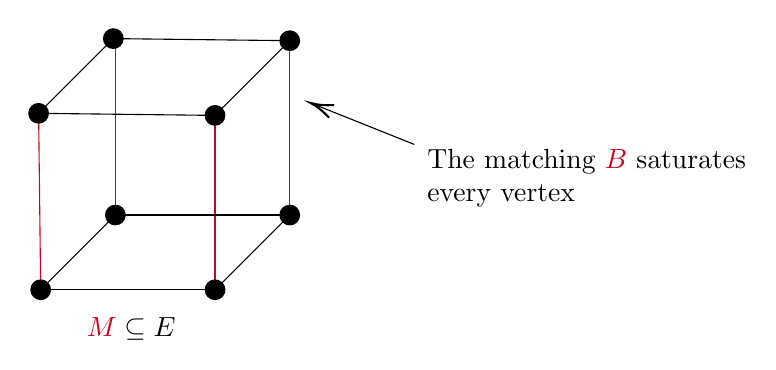
\begin{tikzpicture}[x=0.75pt,y=0.75pt,yscale=-1,xscale=1]
%uncomment if require: \path (0,193); %set diagram left start at 0, and has height of 193

%Straight Lines [id:da805561755073776] 
\draw [color={rgb, 255:red, 208; green, 2; blue, 27 }  ,draw opacity=1 ]   (216,40) -- (216,124) ;
%Straight Lines [id:da4603353852817845] 
\draw [color={rgb, 255:red, 208; green, 2; blue, 27 }  ,draw opacity=1 ]   (264,76) -- (264,160) ;
%Straight Lines [id:da9593359618444844] 
\draw [color={rgb, 255:red, 208; green, 2; blue, 27 }  ,draw opacity=1 ]   (300,40) -- (300,124) ;
%Straight Lines [id:da9136430441630193] 
\draw [color={rgb, 255:red, 208; green, 2; blue, 27 }  ,draw opacity=1 ]   (180,160) -- (179,75) ;
%Straight Lines [id:da752047043089495] 
\draw    (300,124) -- (216,124) ;
%Straight Lines [id:da6627915769720192] 
\draw    (180,160) -- (216,124) ;
%Straight Lines [id:da7505916838885378] 
\draw    (360,90) -- (311.86,70.74) ;
\draw [shift={(310,70)}, rotate = 381.8] [color={rgb, 255:red, 0; green, 0; blue, 0 }  ][line width=0.75]    (10.93,-3.29) .. controls (6.95,-1.4) and (3.31,-0.3) .. (0,0) .. controls (3.31,0.3) and (6.95,1.4) .. (10.93,3.29)   ;
%Shape: Circle [id:dp36912951700681307] 
\draw  [draw opacity=0][fill={rgb, 255:red, 0; green, 0; blue, 0 }  ,fill opacity=1 ] (175,160) .. controls (175,157.24) and (177.24,155) .. (180,155) .. controls (182.76,155) and (185,157.24) .. (185,160) .. controls (185,162.76) and (182.76,165) .. (180,165) .. controls (177.24,165) and (175,162.76) .. (175,160) -- cycle ;
%Shape: Circle [id:dp4704505241972967] 
\draw  [draw opacity=0][fill={rgb, 255:red, 0; green, 0; blue, 0 }  ,fill opacity=1 ] (259,160) .. controls (259,157.24) and (261.24,155) .. (264,155) .. controls (266.76,155) and (269,157.24) .. (269,160) .. controls (269,162.76) and (266.76,165) .. (264,165) .. controls (261.24,165) and (259,162.76) .. (259,160) -- cycle ;
%Shape: Circle [id:dp573647341731309] 
\draw  [draw opacity=0][fill={rgb, 255:red, 0; green, 0; blue, 0 }  ,fill opacity=1 ] (295,124) .. controls (295,121.24) and (297.24,119) .. (300,119) .. controls (302.76,119) and (305,121.24) .. (305,124) .. controls (305,126.76) and (302.76,129) .. (300,129) .. controls (297.24,129) and (295,126.76) .. (295,124) -- cycle ;
%Shape: Circle [id:dp3326458532855674] 
\draw  [draw opacity=0][fill={rgb, 255:red, 0; green, 0; blue, 0 }  ,fill opacity=1 ] (295,40) .. controls (295,37.24) and (297.24,35) .. (300,35) .. controls (302.76,35) and (305,37.24) .. (305,40) .. controls (305,42.76) and (302.76,45) .. (300,45) .. controls (297.24,45) and (295,42.76) .. (295,40) -- cycle ;
%Shape: Circle [id:dp4656041977513993] 
\draw  [draw opacity=0][fill={rgb, 255:red, 0; green, 0; blue, 0 }  ,fill opacity=1 ] (259,76) .. controls (259,73.24) and (261.24,71) .. (264,71) .. controls (266.76,71) and (269,73.24) .. (269,76) .. controls (269,78.76) and (266.76,81) .. (264,81) .. controls (261.24,81) and (259,78.76) .. (259,76) -- cycle ;
%Shape: Circle [id:dp7403175942898133] 
\draw  [draw opacity=0][fill={rgb, 255:red, 0; green, 0; blue, 0 }  ,fill opacity=1 ] (174,75) .. controls (174,72.24) and (176.24,70) .. (179,70) .. controls (181.76,70) and (184,72.24) .. (184,75) .. controls (184,77.76) and (181.76,80) .. (179,80) .. controls (176.24,80) and (174,77.76) .. (174,75) -- cycle ;
%Shape: Circle [id:dp3797103652507142] 
\draw  [draw opacity=0][fill={rgb, 255:red, 0; green, 0; blue, 0 }  ,fill opacity=1 ] (210,39) .. controls (210,36.24) and (212.24,34) .. (215,34) .. controls (217.76,34) and (220,36.24) .. (220,39) .. controls (220,41.76) and (217.76,44) .. (215,44) .. controls (212.24,44) and (210,41.76) .. (210,39) -- cycle ;
%Shape: Circle [id:dp5362787773800174] 
\draw  [draw opacity=0][fill={rgb, 255:red, 0; green, 0; blue, 0 }  ,fill opacity=1 ] (211,124) .. controls (211,121.24) and (213.24,119) .. (216,119) .. controls (218.76,119) and (221,121.24) .. (221,124) .. controls (221,126.76) and (218.76,129) .. (216,129) .. controls (213.24,129) and (211,126.76) .. (211,124) -- cycle ;
%Straight Lines [id:da2121231673256675] 
\draw    (215,39) -- (300,40) ;
%Straight Lines [id:da050391166938102305] 
\draw    (179,75) -- (264,76) ;
%Straight Lines [id:da7012868164712192] 
\draw    (180,160) -- (264,160) ;
%Straight Lines [id:da14338113639691086] 
\draw    (264,160) -- (300,124) ;
%Straight Lines [id:da8236516522079884] 
\draw    (179,75) -- (215,39) ;
%Straight Lines [id:da3281665392341566] 
\draw    (264,76) -- (300,40) ;

% Text Node
\draw (365,91) node [anchor=north west][inner sep=0.75pt]   [align=left] {The matching $\displaystyle \textcolor[rgb]{0.82,0.01,0.11}{B}$ saturates\\every vertex};
% Text Node
\draw (201,172) node [anchor=north west][inner sep=0.75pt]    {$\textcolor[rgb]{0.82,0.01,0.11}{M} \subseteq E$};


\end{tikzpicture}

\end{center}
A matching where every vertex is saturated (such as the above) is known as a \vocab{perfect matching}. However, there is no restriction in general on how many vertices are saturated by a matching.

\section{Matching in Bipartite Graphs}

Matchings are particularly interesting in bipartite graphs. We will be interested in the following question: given a bipartite graph $G = (A \cup B, E)$, when can I find a matching saturating $A$?

\begin{center}
	

\tikzset{every picture/.style={line width=0.75pt}} %set default line width to 0.75pt        

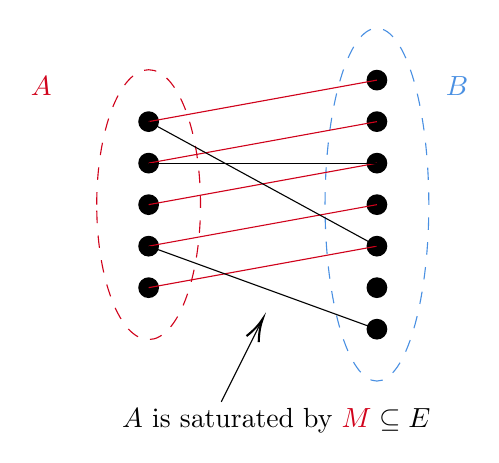
\begin{tikzpicture}[x=0.75pt,y=0.75pt,yscale=-1,xscale=1]
%uncomment if require: \path (0,273); %set diagram left start at 0, and has height of 273

%Straight Lines [id:da7505916838885378] 
\draw    (360,190) -- (379.11,151.79) ;
\draw [shift={(380,150)}, rotate = 476.57] [color={rgb, 255:red, 0; green, 0; blue, 0 }  ][line width=0.75]    (10.93,-3.29) .. controls (6.95,-1.4) and (3.31,-0.3) .. (0,0) .. controls (3.31,0.3) and (6.95,1.4) .. (10.93,3.29)   ;
%Shape: Circle [id:dp36912951700681307] 
\draw  [draw opacity=0][fill={rgb, 255:red, 0; green, 0; blue, 0 }  ,fill opacity=1 ] (320,95) .. controls (320,92.24) and (322.24,90) .. (325,90) .. controls (327.76,90) and (330,92.24) .. (330,95) .. controls (330,97.76) and (327.76,100) .. (325,100) .. controls (322.24,100) and (320,97.76) .. (320,95) -- cycle ;
%Shape: Circle [id:dp44942679974813216] 
\draw  [draw opacity=0][fill={rgb, 255:red, 0; green, 0; blue, 0 }  ,fill opacity=1 ] (320,115) .. controls (320,112.24) and (322.24,110) .. (325,110) .. controls (327.76,110) and (330,112.24) .. (330,115) .. controls (330,117.76) and (327.76,120) .. (325,120) .. controls (322.24,120) and (320,117.76) .. (320,115) -- cycle ;
%Shape: Circle [id:dp6752731223210899] 
\draw  [draw opacity=0][fill={rgb, 255:red, 0; green, 0; blue, 0 }  ,fill opacity=1 ] (320,75) .. controls (320,72.24) and (322.24,70) .. (325,70) .. controls (327.76,70) and (330,72.24) .. (330,75) .. controls (330,77.76) and (327.76,80) .. (325,80) .. controls (322.24,80) and (320,77.76) .. (320,75) -- cycle ;
%Shape: Circle [id:dp4233872987178915] 
\draw  [draw opacity=0][fill={rgb, 255:red, 0; green, 0; blue, 0 }  ,fill opacity=1 ] (320,55) .. controls (320,52.24) and (322.24,50) .. (325,50) .. controls (327.76,50) and (330,52.24) .. (330,55) .. controls (330,57.76) and (327.76,60) .. (325,60) .. controls (322.24,60) and (320,57.76) .. (320,55) -- cycle ;
%Shape: Circle [id:dp04653911603417005] 
\draw  [draw opacity=0][fill={rgb, 255:red, 0; green, 0; blue, 0 }  ,fill opacity=1 ] (320,135) .. controls (320,132.24) and (322.24,130) .. (325,130) .. controls (327.76,130) and (330,132.24) .. (330,135) .. controls (330,137.76) and (327.76,140) .. (325,140) .. controls (322.24,140) and (320,137.76) .. (320,135) -- cycle ;
%Shape: Ellipse [id:dp31141580503923916] 
\draw  [color={rgb, 255:red, 208; green, 2; blue, 27 }  ,draw opacity=1 ][dash pattern={on 4.5pt off 4.5pt}] (300,95) .. controls (300,59.1) and (311.19,30) .. (325,30) .. controls (338.81,30) and (350,59.1) .. (350,95) .. controls (350,130.9) and (338.81,160) .. (325,160) .. controls (311.19,160) and (300,130.9) .. (300,95) -- cycle ;
%Shape: Circle [id:dp6358985628093098] 
\draw  [draw opacity=0][fill={rgb, 255:red, 0; green, 0; blue, 0 }  ,fill opacity=1 ] (430,75) .. controls (430,72.24) and (432.24,70) .. (435,70) .. controls (437.76,70) and (440,72.24) .. (440,75) .. controls (440,77.76) and (437.76,80) .. (435,80) .. controls (432.24,80) and (430,77.76) .. (430,75) -- cycle ;
%Shape: Circle [id:dp880304645428568] 
\draw  [draw opacity=0][fill={rgb, 255:red, 0; green, 0; blue, 0 }  ,fill opacity=1 ] (430,95) .. controls (430,92.24) and (432.24,90) .. (435,90) .. controls (437.76,90) and (440,92.24) .. (440,95) .. controls (440,97.76) and (437.76,100) .. (435,100) .. controls (432.24,100) and (430,97.76) .. (430,95) -- cycle ;
%Shape: Circle [id:dp9506904233850559] 
\draw  [draw opacity=0][fill={rgb, 255:red, 0; green, 0; blue, 0 }  ,fill opacity=1 ] (430,55) .. controls (430,52.24) and (432.24,50) .. (435,50) .. controls (437.76,50) and (440,52.24) .. (440,55) .. controls (440,57.76) and (437.76,60) .. (435,60) .. controls (432.24,60) and (430,57.76) .. (430,55) -- cycle ;
%Shape: Circle [id:dp594682452060607] 
\draw  [draw opacity=0][fill={rgb, 255:red, 0; green, 0; blue, 0 }  ,fill opacity=1 ] (430,35) .. controls (430,32.24) and (432.24,30) .. (435,30) .. controls (437.76,30) and (440,32.24) .. (440,35) .. controls (440,37.76) and (437.76,40) .. (435,40) .. controls (432.24,40) and (430,37.76) .. (430,35) -- cycle ;
%Shape: Circle [id:dp7145369093884492] 
\draw  [draw opacity=0][fill={rgb, 255:red, 0; green, 0; blue, 0 }  ,fill opacity=1 ] (430,115) .. controls (430,112.24) and (432.24,110) .. (435,110) .. controls (437.76,110) and (440,112.24) .. (440,115) .. controls (440,117.76) and (437.76,120) .. (435,120) .. controls (432.24,120) and (430,117.76) .. (430,115) -- cycle ;
%Shape: Ellipse [id:dp7407681681896772] 
\draw  [color={rgb, 255:red, 74; green, 144; blue, 226 }  ,draw opacity=1 ][dash pattern={on 4.5pt off 4.5pt}] (410,95) .. controls (410,48.06) and (421.19,10) .. (435,10) .. controls (448.81,10) and (460,48.06) .. (460,95) .. controls (460,141.94) and (448.81,180) .. (435,180) .. controls (421.19,180) and (410,141.94) .. (410,95) -- cycle ;
%Shape: Circle [id:dp33340512760145824] 
\draw  [draw opacity=0][fill={rgb, 255:red, 0; green, 0; blue, 0 }  ,fill opacity=1 ] (430,135) .. controls (430,132.24) and (432.24,130) .. (435,130) .. controls (437.76,130) and (440,132.24) .. (440,135) .. controls (440,137.76) and (437.76,140) .. (435,140) .. controls (432.24,140) and (430,137.76) .. (430,135) -- cycle ;
%Shape: Circle [id:dp724679030580349] 
\draw  [draw opacity=0][fill={rgb, 255:red, 0; green, 0; blue, 0 }  ,fill opacity=1 ] (430,155) .. controls (430,152.24) and (432.24,150) .. (435,150) .. controls (437.76,150) and (440,152.24) .. (440,155) .. controls (440,157.76) and (437.76,160) .. (435,160) .. controls (432.24,160) and (430,157.76) .. (430,155) -- cycle ;
%Straight Lines [id:da6673725902420062] 
\draw [color={rgb, 255:red, 208; green, 2; blue, 27 }  ,draw opacity=1 ]   (325,55) -- (435,35) ;
%Straight Lines [id:da4203133178921782] 
\draw [color={rgb, 255:red, 208; green, 2; blue, 27 }  ,draw opacity=1 ]   (325,75) -- (435,55) ;
%Straight Lines [id:da16049164399667892] 
\draw [color={rgb, 255:red, 208; green, 2; blue, 27 }  ,draw opacity=1 ]   (325,95) -- (435,75) ;
%Straight Lines [id:da19642811620000844] 
\draw [color={rgb, 255:red, 208; green, 2; blue, 27 }  ,draw opacity=1 ]   (325,115) -- (435,95) ;
%Straight Lines [id:da21466460093090467] 
\draw [color={rgb, 255:red, 208; green, 2; blue, 27 }  ,draw opacity=1 ]   (325,135) -- (435,115) ;
%Straight Lines [id:da04929331633411782] 
\draw    (325,115) -- (435,155) ;
%Straight Lines [id:da7611641968859248] 
\draw    (325,75) -- (435,75) ;
%Straight Lines [id:da5620035391275132] 
\draw    (325,55) -- (435,115) ;

% Text Node
\draw (311,192) node [anchor=north west][inner sep=0.75pt]   [align=left] {$\displaystyle A$ is saturated by $\displaystyle \textcolor[rgb]{0.82,0.01,0.11}{M} \subseteq E$};
% Text Node
\draw (267,32) node [anchor=north west][inner sep=0.75pt]    {$\textcolor[rgb]{0.82,0.01,0.11}{A}$};
% Text Node
\draw (467,32) node [anchor=north west][inner sep=0.75pt]  [color={rgb, 255:red, 74; green, 144; blue, 226 }  ,opacity=1 ]  {$B$};


\end{tikzpicture}
\end{center}

This question is the same as asking when is there a function $f: A \rightarrow B$ where $xf(x) \in E$ that is in injection.

In trying to answer this question, we might try and think about why it may not be possible. The simplest reason is when $B$ isn't large enough to have an injection, when $|B| \leq |A|$. In a similar way, we might have a graph is big enough, but that isn't true for a small part of the graph, like below.
\begin{center}
	

\tikzset{every picture/.style={line width=0.75pt}} %set default line width to 0.75pt        

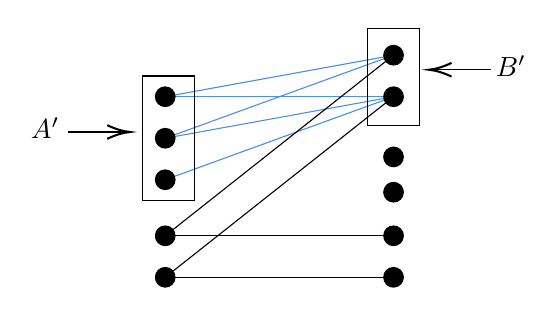
\begin{tikzpicture}[x=0.75pt,y=0.75pt,yscale=-1,xscale=1]
%uncomment if require: \path (0,273); %set diagram left start at 0, and has height of 273

%Straight Lines [id:da8369400892067791] 
\draw    (324,130) -- (434,130) ;
%Straight Lines [id:da19495235143878997] 
\draw    (324,150) -- (434,150) ;
%Straight Lines [id:da40390592166983896] 
\draw [color={rgb, 255:red, 74; green, 144; blue, 226 }  ,draw opacity=1 ]   (324,63) -- (434,43) ;
%Straight Lines [id:da3965802064481285] 
\draw [color={rgb, 255:red, 74; green, 144; blue, 226 }  ,draw opacity=1 ]   (324,83) -- (434,43) ;
%Straight Lines [id:da6637904851386653] 
\draw [color={rgb, 255:red, 74; green, 144; blue, 226 }  ,draw opacity=1 ]   (324,103) -- (434,63) ;
%Straight Lines [id:da1589473171205299] 
\draw [color={rgb, 255:red, 74; green, 144; blue, 226 }  ,draw opacity=1 ]   (324,83) -- (434,63) ;
%Straight Lines [id:da6181500242724567] 
\draw [color={rgb, 255:red, 74; green, 144; blue, 226 }  ,draw opacity=1 ]   (324,63) -- (434,63) ;
%Straight Lines [id:da7181423353650153] 
\draw    (324,130) -- (434,43) ;
%Straight Lines [id:da38882946887707004] 
\draw    (324,150) -- (434,63) ;
%Shape: Circle [id:dp42681003962364517] 
\draw  [draw opacity=0][fill={rgb, 255:red, 0; green, 0; blue, 0 }  ,fill opacity=1 ] (319,103) .. controls (319,100.24) and (321.24,98) .. (324,98) .. controls (326.76,98) and (329,100.24) .. (329,103) .. controls (329,105.76) and (326.76,108) .. (324,108) .. controls (321.24,108) and (319,105.76) .. (319,103) -- cycle ;
%Shape: Circle [id:dp04672707446321711] 
\draw  [draw opacity=0][fill={rgb, 255:red, 0; green, 0; blue, 0 }  ,fill opacity=1 ] (319,130) .. controls (319,127.24) and (321.24,125) .. (324,125) .. controls (326.76,125) and (329,127.24) .. (329,130) .. controls (329,132.76) and (326.76,135) .. (324,135) .. controls (321.24,135) and (319,132.76) .. (319,130) -- cycle ;
%Shape: Circle [id:dp6968869451584372] 
\draw  [draw opacity=0][fill={rgb, 255:red, 0; green, 0; blue, 0 }  ,fill opacity=1 ] (319,83) .. controls (319,80.24) and (321.24,78) .. (324,78) .. controls (326.76,78) and (329,80.24) .. (329,83) .. controls (329,85.76) and (326.76,88) .. (324,88) .. controls (321.24,88) and (319,85.76) .. (319,83) -- cycle ;
%Shape: Circle [id:dp5397070239729519] 
\draw  [draw opacity=0][fill={rgb, 255:red, 0; green, 0; blue, 0 }  ,fill opacity=1 ] (319,63) .. controls (319,60.24) and (321.24,58) .. (324,58) .. controls (326.76,58) and (329,60.24) .. (329,63) .. controls (329,65.76) and (326.76,68) .. (324,68) .. controls (321.24,68) and (319,65.76) .. (319,63) -- cycle ;
%Shape: Circle [id:dp1933015038500212] 
\draw  [draw opacity=0][fill={rgb, 255:red, 0; green, 0; blue, 0 }  ,fill opacity=1 ] (319,150) .. controls (319,147.24) and (321.24,145) .. (324,145) .. controls (326.76,145) and (329,147.24) .. (329,150) .. controls (329,152.76) and (326.76,155) .. (324,155) .. controls (321.24,155) and (319,152.76) .. (319,150) -- cycle ;
%Shape: Circle [id:dp22027602623518294] 
\draw  [draw opacity=0][fill={rgb, 255:red, 0; green, 0; blue, 0 }  ,fill opacity=1 ] (429,92) .. controls (429,89.24) and (431.24,87) .. (434,87) .. controls (436.76,87) and (439,89.24) .. (439,92) .. controls (439,94.76) and (436.76,97) .. (434,97) .. controls (431.24,97) and (429,94.76) .. (429,92) -- cycle ;
%Shape: Circle [id:dp6065822004480979] 
\draw  [draw opacity=0][fill={rgb, 255:red, 0; green, 0; blue, 0 }  ,fill opacity=1 ] (429,109) .. controls (429,106.24) and (431.24,104) .. (434,104) .. controls (436.76,104) and (439,106.24) .. (439,109) .. controls (439,111.76) and (436.76,114) .. (434,114) .. controls (431.24,114) and (429,111.76) .. (429,109) -- cycle ;
%Shape: Circle [id:dp8722990507351452] 
\draw  [draw opacity=0][fill={rgb, 255:red, 0; green, 0; blue, 0 }  ,fill opacity=1 ] (429,63) .. controls (429,60.24) and (431.24,58) .. (434,58) .. controls (436.76,58) and (439,60.24) .. (439,63) .. controls (439,65.76) and (436.76,68) .. (434,68) .. controls (431.24,68) and (429,65.76) .. (429,63) -- cycle ;
%Shape: Circle [id:dp6972009025737637] 
\draw  [draw opacity=0][fill={rgb, 255:red, 0; green, 0; blue, 0 }  ,fill opacity=1 ] (429,43) .. controls (429,40.24) and (431.24,38) .. (434,38) .. controls (436.76,38) and (439,40.24) .. (439,43) .. controls (439,45.76) and (436.76,48) .. (434,48) .. controls (431.24,48) and (429,45.76) .. (429,43) -- cycle ;
%Shape: Circle [id:dp036260952386616085] 
\draw  [draw opacity=0][fill={rgb, 255:red, 0; green, 0; blue, 0 }  ,fill opacity=1 ] (429,130) .. controls (429,127.24) and (431.24,125) .. (434,125) .. controls (436.76,125) and (439,127.24) .. (439,130) .. controls (439,132.76) and (436.76,135) .. (434,135) .. controls (431.24,135) and (429,132.76) .. (429,130) -- cycle ;
%Shape: Circle [id:dp3214854269825461] 
\draw  [draw opacity=0][fill={rgb, 255:red, 0; green, 0; blue, 0 }  ,fill opacity=1 ] (429,150) .. controls (429,147.24) and (431.24,145) .. (434,145) .. controls (436.76,145) and (439,147.24) .. (439,150) .. controls (439,152.76) and (436.76,155) .. (434,155) .. controls (431.24,155) and (429,152.76) .. (429,150) -- cycle ;
%Shape: Rectangle [id:dp8613689383791837] 
\draw   (313,53) -- (338,53) -- (338,113) -- (313,113) -- cycle ;
%Shape: Rectangle [id:dp49091409543282016] 
\draw   (421.5,30) -- (446.5,30) -- (446.5,77) -- (421.5,77) -- cycle ;
%Straight Lines [id:da8087602747586281] 
\draw    (277,80) -- (305,80) ;
\draw [shift={(307,80)}, rotate = 180] [color={rgb, 255:red, 0; green, 0; blue, 0 }  ][line width=0.75]    (10.93,-3.29) .. controls (6.95,-1.4) and (3.31,-0.3) .. (0,0) .. controls (3.31,0.3) and (6.95,1.4) .. (10.93,3.29)   ;
%Straight Lines [id:da9186974784747017] 
\draw    (481,50) -- (453,50) ;
\draw [shift={(451,50)}, rotate = 360] [color={rgb, 255:red, 0; green, 0; blue, 0 }  ][line width=0.75]    (10.93,-3.29) .. controls (6.95,-1.4) and (3.31,-0.3) .. (0,0) .. controls (3.31,0.3) and (6.95,1.4) .. (10.93,3.29)   ;

% Text Node
\draw (258,72) node [anchor=north west][inner sep=0.75pt]    {$A'$};
% Text Node
\draw (482,42) node [anchor=north west][inner sep=0.75pt]    {$B'$};


\end{tikzpicture}

\end{center}
What Hall's theorem says is that this issue is the only obstruction to creating such a matching. 

\begin{definition}[Neighbourhood of a Vertex Set]
	If $X \subseteq V$, then we define $N(X)$, the \vocab{neighbourhood of $X$} to be $\displaystyle N(X) = \bigcup_{x \in X} N(x)$.
\end{definition}

With the notion of the neighborhood of a set of vertices, we can rephrase the issue mentioned about as $|N(A')| < |A'|$ for some subset $A' \subseteq A$. We will use this notation in our statement for Hall's theorem.

Before we prove the theorem, we will need to prepare a little bit.

\begin{definition}[$M$-Alternating Path]
	Let $G = (V, E)$ be a graph with a matching $M$ in $G$. We say that a path $P = x_1 \dots x_l$ is \vocab{M-alternating} if $x_i x_{i + 1}$ is alternately in $M$ and not in $M$.
\end{definition}

\begin{center}
	

\tikzset{every picture/.style={line width=0.75pt}} %set default line width to 0.75pt        

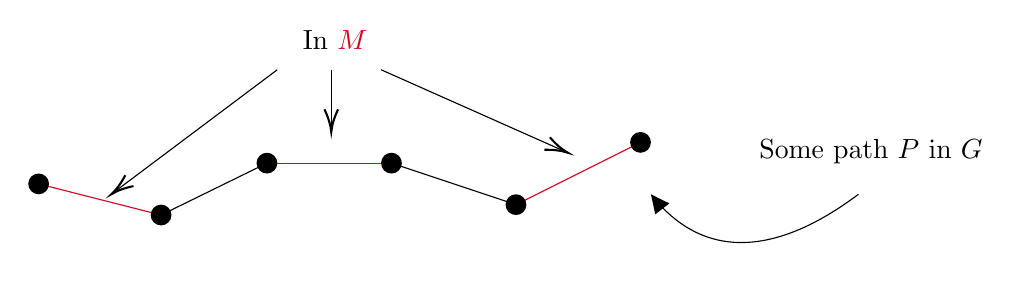
\begin{tikzpicture}[x=0.75pt,y=0.75pt,yscale=-1,xscale=1]
%uncomment if require: \path (0,273); %set diagram left start at 0, and has height of 273

%Straight Lines [id:da1911727766997673] 
\draw    (324,130) -- (375,105) ;
%Straight Lines [id:da41633838448849425] 
\draw [color={rgb, 255:red, 208; green, 2; blue, 27 }  ,draw opacity=1 ]   (375,105) -- (435,105) ;
%Straight Lines [id:da6472416846171128] 
\draw    (435,105) -- (495,125) ;
%Straight Lines [id:da8981575716010599] 
\draw [color={rgb, 255:red, 208; green, 2; blue, 27 }  ,draw opacity=1 ]   (495,125) -- (555,95) ;
%Straight Lines [id:da7701616382388665] 
\draw [color={rgb, 255:red, 208; green, 2; blue, 27 }  ,draw opacity=1 ]   (324,130) -- (265,115) ;
%Shape: Circle [id:dp7703800629553158] 
\draw  [draw opacity=0][fill={rgb, 255:red, 0; green, 0; blue, 0 }  ,fill opacity=1 ] (319,130) .. controls (319,127.24) and (321.24,125) .. (324,125) .. controls (326.76,125) and (329,127.24) .. (329,130) .. controls (329,132.76) and (326.76,135) .. (324,135) .. controls (321.24,135) and (319,132.76) .. (319,130) -- cycle ;
%Shape: Circle [id:dp0226725339534235] 
\draw  [draw opacity=0][fill={rgb, 255:red, 0; green, 0; blue, 0 }  ,fill opacity=1 ] (370,105) .. controls (370,102.24) and (372.24,100) .. (375,100) .. controls (377.76,100) and (380,102.24) .. (380,105) .. controls (380,107.76) and (377.76,110) .. (375,110) .. controls (372.24,110) and (370,107.76) .. (370,105) -- cycle ;
%Shape: Circle [id:dp34568978664728356] 
\draw  [draw opacity=0][fill={rgb, 255:red, 0; green, 0; blue, 0 }  ,fill opacity=1 ] (430,105) .. controls (430,102.24) and (432.24,100) .. (435,100) .. controls (437.76,100) and (440,102.24) .. (440,105) .. controls (440,107.76) and (437.76,110) .. (435,110) .. controls (432.24,110) and (430,107.76) .. (430,105) -- cycle ;
%Shape: Circle [id:dp8179415147207098] 
\draw  [draw opacity=0][fill={rgb, 255:red, 0; green, 0; blue, 0 }  ,fill opacity=1 ] (490,125) .. controls (490,122.24) and (492.24,120) .. (495,120) .. controls (497.76,120) and (500,122.24) .. (500,125) .. controls (500,127.76) and (497.76,130) .. (495,130) .. controls (492.24,130) and (490,127.76) .. (490,125) -- cycle ;
%Shape: Circle [id:dp0812463035943316] 
\draw  [draw opacity=0][fill={rgb, 255:red, 0; green, 0; blue, 0 }  ,fill opacity=1 ] (550,95) .. controls (550,92.24) and (552.24,90) .. (555,90) .. controls (557.76,90) and (560,92.24) .. (560,95) .. controls (560,97.76) and (557.76,100) .. (555,100) .. controls (552.24,100) and (550,97.76) .. (550,95) -- cycle ;
%Shape: Circle [id:dp412793926190299] 
\draw  [draw opacity=0][fill={rgb, 255:red, 0; green, 0; blue, 0 }  ,fill opacity=1 ] (260,115) .. controls (260,112.24) and (262.24,110) .. (265,110) .. controls (267.76,110) and (270,112.24) .. (270,115) .. controls (270,117.76) and (267.76,120) .. (265,120) .. controls (262.24,120) and (260,117.76) .. (260,115) -- cycle ;
%Straight Lines [id:da524865354422517] 
\draw    (380,60) -- (301.6,118.8) ;
\draw [shift={(300,120)}, rotate = 323.13] [color={rgb, 255:red, 0; green, 0; blue, 0 }  ][line width=0.75]    (10.93,-3.29) .. controls (6.95,-1.4) and (3.31,-0.3) .. (0,0) .. controls (3.31,0.3) and (6.95,1.4) .. (10.93,3.29)   ;
%Straight Lines [id:da3699327393316867] 
\draw    (406,60) -- (406,88) ;
\draw [shift={(406,90)}, rotate = 270] [color={rgb, 255:red, 0; green, 0; blue, 0 }  ][line width=0.75]    (10.93,-3.29) .. controls (6.95,-1.4) and (3.31,-0.3) .. (0,0) .. controls (3.31,0.3) and (6.95,1.4) .. (10.93,3.29)   ;
%Straight Lines [id:da39528029770693984] 
\draw    (430,60) -- (518.17,99.19) ;
\draw [shift={(520,100)}, rotate = 203.96] [color={rgb, 255:red, 0; green, 0; blue, 0 }  ][line width=0.75]    (10.93,-3.29) .. controls (6.95,-1.4) and (3.31,-0.3) .. (0,0) .. controls (3.31,0.3) and (6.95,1.4) .. (10.93,3.29)   ;
%Curve Lines [id:da07952038804691897] 
\draw    (561.89,122.34) .. controls (586.75,151.88) and (621,149.25) .. (660,120) ;
\draw [shift={(560,120)}, rotate = 52] [fill={rgb, 255:red, 0; green, 0; blue, 0 }  ][line width=0.08]  [draw opacity=0] (8.93,-4.29) -- (0,0) -- (8.93,4.29) -- cycle    ;

% Text Node
\draw (391,40) node [anchor=north west][inner sep=0.75pt]   [align=left] {In $\displaystyle \textcolor[rgb]{0.82,0.01,0.11}{M}$};
% Text Node
\draw (611,92) node [anchor=north west][inner sep=0.75pt]   [align=left] {Some path $\displaystyle P$ in $\displaystyle G$};


\end{tikzpicture}

\end{center}

Another example of an $M$-alternating path is the one below.
\begin{center}
	

\tikzset{every picture/.style={line width=0.75pt}} %set default line width to 0.75pt        

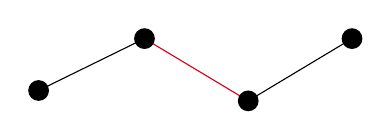
\begin{tikzpicture}[x=0.75pt,y=0.75pt,yscale=-1,xscale=1]
%uncomment if require: \path (0,273); %set diagram left start at 0, and has height of 273

%Straight Lines [id:da6545369317269095] 
\draw    (324,130) -- (375,105) ;
%Straight Lines [id:da5998112575007682] 
\draw [color={rgb, 255:red, 208; green, 2; blue, 27 }  ,draw opacity=1 ]   (375,105) -- (425,135) ;
%Straight Lines [id:da3813029402731277] 
\draw    (425,135) -- (475,105) ;
%Shape: Circle [id:dp4518952685232853] 
\draw  [draw opacity=0][fill={rgb, 255:red, 0; green, 0; blue, 0 }  ,fill opacity=1 ] (319,130) .. controls (319,127.24) and (321.24,125) .. (324,125) .. controls (326.76,125) and (329,127.24) .. (329,130) .. controls (329,132.76) and (326.76,135) .. (324,135) .. controls (321.24,135) and (319,132.76) .. (319,130) -- cycle ;
%Shape: Circle [id:dp4872392702945506] 
\draw  [draw opacity=0][fill={rgb, 255:red, 0; green, 0; blue, 0 }  ,fill opacity=1 ] (370,105) .. controls (370,102.24) and (372.24,100) .. (375,100) .. controls (377.76,100) and (380,102.24) .. (380,105) .. controls (380,107.76) and (377.76,110) .. (375,110) .. controls (372.24,110) and (370,107.76) .. (370,105) -- cycle ;
%Shape: Circle [id:dp8339741130332603] 
\draw  [draw opacity=0][fill={rgb, 255:red, 0; green, 0; blue, 0 }  ,fill opacity=1 ] (420,135) .. controls (420,132.24) and (422.24,130) .. (425,130) .. controls (427.76,130) and (430,132.24) .. (430,135) .. controls (430,137.76) and (427.76,140) .. (425,140) .. controls (422.24,140) and (420,137.76) .. (420,135) -- cycle ;
%Shape: Circle [id:dp6104072071427933] 
\draw  [draw opacity=0][fill={rgb, 255:red, 0; green, 0; blue, 0 }  ,fill opacity=1 ] (470,105) .. controls (470,102.24) and (472.24,100) .. (475,100) .. controls (477.76,100) and (480,102.24) .. (480,105) .. controls (480,107.76) and (477.76,110) .. (475,110) .. controls (472.24,110) and (470,107.76) .. (470,105) -- cycle ;




\end{tikzpicture}

\end{center}
If we saw the path above in the graph, and we knew that the end vertices was not saturated, then we could change the edges that are in $M$, so we would still have a matching. This move will be key in our proof of Hall's theorem.
\begin{center}
	

\tikzset{every picture/.style={line width=0.75pt}} %set default line width to 0.75pt        

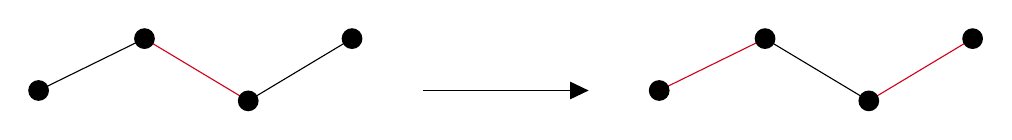
\begin{tikzpicture}[x=0.75pt,y=0.75pt,yscale=-1,xscale=1]
%uncomment if require: \path (0,273); %set diagram left start at 0, and has height of 273

%Straight Lines [id:da8888863291662378] 
\draw    (85,130) -- (136,105) ;
%Straight Lines [id:da2469822147132278] 
\draw [color={rgb, 255:red, 208; green, 2; blue, 27 }  ,draw opacity=1 ]   (136,105) -- (186,135) ;
%Straight Lines [id:da728605608255147] 
\draw    (186,135) -- (236,105) ;
%Shape: Circle [id:dp4177428980499841] 
\draw  [draw opacity=0][fill={rgb, 255:red, 0; green, 0; blue, 0 }  ,fill opacity=1 ] (80,130) .. controls (80,127.24) and (82.24,125) .. (85,125) .. controls (87.76,125) and (90,127.24) .. (90,130) .. controls (90,132.76) and (87.76,135) .. (85,135) .. controls (82.24,135) and (80,132.76) .. (80,130) -- cycle ;
%Shape: Circle [id:dp6460331997754131] 
\draw  [draw opacity=0][fill={rgb, 255:red, 0; green, 0; blue, 0 }  ,fill opacity=1 ] (131,105) .. controls (131,102.24) and (133.24,100) .. (136,100) .. controls (138.76,100) and (141,102.24) .. (141,105) .. controls (141,107.76) and (138.76,110) .. (136,110) .. controls (133.24,110) and (131,107.76) .. (131,105) -- cycle ;
%Shape: Circle [id:dp645196452335059] 
\draw  [draw opacity=0][fill={rgb, 255:red, 0; green, 0; blue, 0 }  ,fill opacity=1 ] (181,135) .. controls (181,132.24) and (183.24,130) .. (186,130) .. controls (188.76,130) and (191,132.24) .. (191,135) .. controls (191,137.76) and (188.76,140) .. (186,140) .. controls (183.24,140) and (181,137.76) .. (181,135) -- cycle ;
%Shape: Circle [id:dp5500348242602249] 
\draw  [draw opacity=0][fill={rgb, 255:red, 0; green, 0; blue, 0 }  ,fill opacity=1 ] (231,105) .. controls (231,102.24) and (233.24,100) .. (236,100) .. controls (238.76,100) and (241,102.24) .. (241,105) .. controls (241,107.76) and (238.76,110) .. (236,110) .. controls (233.24,110) and (231,107.76) .. (231,105) -- cycle ;
%Straight Lines [id:da04862323828569037] 
\draw [color={rgb, 255:red, 208; green, 2; blue, 27 }  ,draw opacity=1 ]   (384,130) -- (435,105) ;
%Straight Lines [id:da8593276291450644] 
\draw [color={rgb, 255:red, 0; green, 0; blue, 0 }  ,draw opacity=1 ]   (435,105) -- (485,135) ;
%Straight Lines [id:da2442782076245853] 
\draw [color={rgb, 255:red, 208; green, 2; blue, 27 }  ,draw opacity=1 ]   (485,135) -- (535,105) ;
%Shape: Circle [id:dp8967679325781175] 
\draw  [draw opacity=0][fill={rgb, 255:red, 0; green, 0; blue, 0 }  ,fill opacity=1 ] (379,130) .. controls (379,127.24) and (381.24,125) .. (384,125) .. controls (386.76,125) and (389,127.24) .. (389,130) .. controls (389,132.76) and (386.76,135) .. (384,135) .. controls (381.24,135) and (379,132.76) .. (379,130) -- cycle ;
%Shape: Circle [id:dp02900574109663423] 
\draw  [draw opacity=0][fill={rgb, 255:red, 0; green, 0; blue, 0 }  ,fill opacity=1 ] (430,105) .. controls (430,102.24) and (432.24,100) .. (435,100) .. controls (437.76,100) and (440,102.24) .. (440,105) .. controls (440,107.76) and (437.76,110) .. (435,110) .. controls (432.24,110) and (430,107.76) .. (430,105) -- cycle ;
%Shape: Circle [id:dp6936458928095013] 
\draw  [draw opacity=0][fill={rgb, 255:red, 0; green, 0; blue, 0 }  ,fill opacity=1 ] (480,135) .. controls (480,132.24) and (482.24,130) .. (485,130) .. controls (487.76,130) and (490,132.24) .. (490,135) .. controls (490,137.76) and (487.76,140) .. (485,140) .. controls (482.24,140) and (480,137.76) .. (480,135) -- cycle ;
%Shape: Circle [id:dp8748230047935752] 
\draw  [draw opacity=0][fill={rgb, 255:red, 0; green, 0; blue, 0 }  ,fill opacity=1 ] (530,105) .. controls (530,102.24) and (532.24,100) .. (535,100) .. controls (537.76,100) and (540,102.24) .. (540,105) .. controls (540,107.76) and (537.76,110) .. (535,110) .. controls (532.24,110) and (530,107.76) .. (530,105) -- cycle ;
%Straight Lines [id:da7535818285708197] 
\draw    (270,130) -- (347,130) ;
\draw [shift={(350,130)}, rotate = 180] [fill={rgb, 255:red, 0; green, 0; blue, 0 }  ][line width=0.08]  [draw opacity=0] (8.93,-4.29) -- (0,0) -- (8.93,4.29) -- cycle    ;




\end{tikzpicture}

\end{center}
We are going to call this configuration an \emph{augmented path}.

\begin{definition}[$M$-Augmenting Path]
	Given a graph $G = (V, E)$ and a matching $M$ in $G$, an $M$-alternating path $P = x_1 \dots x_l$ is said to be \vocab{$M$-augmenting} if $x_1$ and $x_l$ are not saturated.
\end{definition}
\begin{proposition}
	If $M$ is a matching in $G$ of maximum size, then there are no $M$-augmenting paths.
\end{proposition}
\begin{proof}
	If there is an $M$-augmenting path in $G$, then we can flip the edges of $M$ along $P$ to find a strictly larger matching.
\end{proof}

An important observation is that an $M$-alternating path in a bipartite graph $G = (A\cup B, E)$ with $P = x_1 \dots x_l$, with $x_1 \in A$ and $x_1 x_2 \in M$, then $x_{2k + 1}x_{2k + 2} \in M$, and vice versa.

\section{Hall's Theorem}

We are now ready to state and proof Hall's matching theorem, which formalises the ideas mentioned in the previous section.

\begin{theorem}[Hall's Theorem]
	Let $G = (A \cup B, E)$ be a bipartite graph. Then there exists a matching saturating $A$ if and only if every subset $A' \subseteq A$ satisfies $|N(A')| \geq |A'|$.
\end{theorem}
\begin{proof}
	First we prove the forward (and easy) direction. Let $A' = \{x_1, \dots, x_t \} \subseteq A$. We have matching edges $x_1 y_1, \dots, x_t y_t \in M \subseteq E$, and thus $\{y_1, \dots, y_t\} \subseteq N(A')$, and thus $|N(A')| \geq |A'|$.

	Now for the other (harder) direction, which is that this condition implies the existence of such a matching. Choose a matching $M$ in $G$ with $|M|$ maximized. For a contradiction, assume there is some vertex $a_0 \in A$ that is not saturated by $M$.

	We inductively define sets $A_i \subseteq A$, $B_t \subseteq B$ by setting $A_0 = \{a_0\}$, $B_0 = \emptyset$. We will maintain, for all $t$, that
	\begin{enumerate}
		\item $|A_t| = t + 1$, $|B_t| = t$.
		\item Every vertex in $A_t \cup B_t$ is the endpoint of an alternating path that started at $a_0$. 
		\item $A_t \backslash \{a_0\}$ is matched to $B_t$.
	\end{enumerate}
	So given $A_t$, $B_t$, we need to define $A_{t + 1}$, $B_{t + 1}$.

	First consider $N(A_t)$. We have $|N(A_t)| \geq |A_t| = t + 1 > |B_t|$. So $N(A_t) \backslash B_t$ is non-empty. So let $b_{t + 1} \in N(A_t) \backslash B_t$. Observe that $b_{t + 1}$ can be reached along an alternating path which started at $a_0$. Call $y \in A_t$ such that $yb_{t + 1} \in E$. Then $y$ can be reached along an alternating path starting at $a_0$. Let $P = a_0 x_1 \dots x_l y$ be such an alternating path. Since $a_0x_1 \not \in M$, $x_l y \in M$. Hence $Pb_{t + 1}$ is a alternating path.

	Now, $b_{t + 1}$ is saturated by $M$, as otherwise $Pb_{t + 1}$ would be an $M$-augmenting path, which is a contradiction. So let $a_{t+1}b_{t+1} \in M$. We claim $a_{t + 1} \not \in A_t$, since $A_t$ is matched to $B_t$, and $b_{t + 1} \not \in B_t$. So we may define $A_{t + 1} = A_t \cup \{a_{t + 1}\}$ and $B_{t + 1} = B_t \cup \{b_{t + 1}\}$. We can check that what we claimed before holds. 

	Since $a_{t + 1} \not \in A_t$, and $b_{t + 1} \not \in B_t$, we have $|A_{t +1}| = |A_t| + 1$ and $|B_{t + 1}| = |B_t| + 1$. Also every vertex is the endpoint of an alternating path starting at $a_0$ by construction. Also $A_{t + 1}\backslash\{a_0\}$ is matched to $B_{t + 1}$ since $A_t\backslash\{a_0\}$ is matched to $B_t$, and by construction.

	This completes the construction of $A_t$, $B_t$ for all $t$. Then if $t > |A|$, then $|A_t| > |A|$, but $A_t \subseteq A$, which is a contradiction.
\end{proof}

% Let's look back at the proof in a more informal way. What we did is we started by choosing a maximal sized matching $M$, and we assumed there was some vertex $x_0$ not saturated by $M$.

% What we then did was isolate all of the non-saturated vertices in the graph.

\end{document} 
